% !BIB TS-program = biber
%--------------------
% Packages
% -------------------
\documentclass[11pt,a4paper]{article}

\usepackage{mathptmx} % Use Times Font
\usepackage{times}
\usepackage{amsmath}
\usepackage[style=authoryear,backend=biber]{biblatex} %Imports biblatex package

\addbibresource{ref.bib}
\usepackage[pdftex]{graphicx} % Required for including pictures
\usepackage[pdftex,linkcolor=black,pdfborder={0 0 0}]{hyperref} % Format links for pdf
\usepackage{calc} % To reset the counter in the document after title page
\usepackage{enumitem} % Includes lists
\usepackage{booktabs}
\frenchspacing % No double spacing between sentences
\linespread{1.2} % Set linespace
\usepackage[a4paper, lmargin=0.1666\paperwidth, rmargin=0.1666\paperwidth, tmargin=0.1111\paperheight, bmargin=0.1111\paperheight]{geometry} %margins
%\usepackage{parskip}

\usepackage[all]{nowidow} % Tries to remove widows
\usepackage[protrusion=true,expansion=true]{microtype} % Improves typography, load after fontpackage is selected




%-----------------------
% Set pdf information and add title, fill in the fields
%-----------------------
\hypersetup{ 	
pdfsubject = {},
pdftitle = {},
pdfauthor = {}
}
\title{Attribution of the  extreme precipitation related to the August 12th 2020 Carmont, Scotland derailment.}
\author{Simon Tett, School of Geosciences, University of Edinburgh}

%-----------------------
% Begin document
%-----------------------
\begin{document}
\maketitle
\graphicspath{{../figures/}}
\begin{abstract}
	The UK's Convective Permitting Model suggests, in the Stonehaven area, that extreme hourly rainfall changes at Clausius–Clapton +50\%. This leads to an increased probability, relative to late 19th century conditions,  of rainfall similar to the rain that was associated with the fatal rail accident in Carmont on August 12th 2020, by about 30\% with a doubling of probability for such events in a +2K warmer world. Some characteristics of the simulated extreme rain evaluate well against radar values but the  simulated rainfall is about 20-30\% larger than the radar rainfall. This may reflect model problems or shortcomings in  radar  calibration. 
\end{abstract}

\section{Introduction}

On August 12th 2020 a passenger train running from Aberdeen to Glasgow derailed at Carmont near Stonehaven. The train was lightly loaded due to COVID restrictions but three people died and the remaining six people on the train  were injured. The proximate cause of the derailment was gravel being washed out of a drain \parencite{carmontReport2024}. Radar estimates of  rain at 1km x 1km resolution was 51.5 mm of rain falling between 05:50 to 09:00 which was estimated at around a 1-in-a-100 year event. The drain should have been able to deal with that volume of water but because the drain had not been built to design requirements gravel and other debris was washed out of it and onto the tracks. This in turn caused the derailment.

Theory\parencite{allen02insight} suggests that extreme rainfall occurs when the entire column of atmospheric water precipitates. This, in turn,  suggests that extreme precipitation increases fractionally at the same rate as saturated humidity, or for fixed atmospheric pressure, saturated vapour pressure (Clausius-Clapyron; CC). This is about 7\%/K. However, some studies suggest that sub-daily extreme rainfall  could increase  at rates  up to twice CC\parencite{Kendon_Fischer_Short_2023}. WHAT OTHER EVENT ATTRIBUTION OF SUB-DAILY DATA BEEN DONE.

 The goal of this study is to develop the methodology of  \textcite{tett2023edinburgh}  to estimate extreme rainfall return periods for the current climate and change in return period, and rain fall intensity, due to climate change since the late 19th century. This allows us to estimate how much climate change has changed the probability of the Carmont rainfall.
 
   As part of the UKCP18 project\parencite{ukcp2019cpm} a 12 member ensemble from 1980 to 2080, at a resolution of 2.2 km, was ran.  This ensemble, unfortunately, has a software error which occurs when raining systems are advected exactly along the model grid.  Data, after filtering out the impact of this error, are used to estimate how extreme rainfall




\section{Rail Accident Inquiry Findings}\label{sec:stonederail}
In the morning of the 12th of August 2020,
after several hours of extreme rainfall,
the 06:38 service from Aberdeen to Glasgow travelled past Carmont,
between Stonehaven and Montrose.
Due to a landslip reported ahead,
the train reverses to return to Stonehaven.
On this journey,
the train impacts debris washed out from a drain.
The train derailed,
resulting in three fatalities,
with the other six passengers being injured.

As per the Rail Accident Investigation Branch report on the event~\parencite{RAIB_2022},
the extreme rainfall caused flows of surface water that the drain was unable to safely manage.
The RAIB report was created with the intention of preventing railway accidents by finding the causal
factors contributing to the Stonehaven Derailment that are under the control of the railway
and those associated with it.
Therefore,
the report finds that the causal factors are that the drain was not designed to specification
and that railway operations did not fully account for the risks posed by the extreme rainfall.
However,
as the crash was caused by an extreme weather event,
there is a potential additional human-driven causal factor, Anthropogenic Climate Change.

Due to the COVID-19 pandemic,
the train had an extremely low loading of only nine people.
Had this not been the case,
it has been estimated (\cite{RAIB_2022} para. 461) that between 25 and 50 passengers would have been on the train,
which had a capacity of around 300.
With this larger passenger loading,
the derailment would have resulted in a far higher number of casualties,
although the potential number of casualties cannot be assumed due to the variability of casualty risk throughout the train.

A report released by the UK Government in the aftermath of the derailment~\cite{NR_DfT_2021}
was made to discuss the resilience of the UK's rail infrastructure.
This report notes that the signal of climate change is becoming more significant,
and dedicates a section to the impacts climate change will have on rail infrastructure.
It is with this consideration that the attribution analysis for the Stonehaven Event is performed here.

This analysis will proceed by considering the rainfall as the cause of the event.
As the modelling necessary for either the landslip or the drain debris washout is beyond the scope of this report,
the intensity of the extreme rainfall itself will be used to define the event.

\section{Rainfall in a warmer world}\label{sec:warmerrainfall}

It is reasonable to expect that climate change had an impact on the extreme rainfall on 12 August 2020.
One example of this in the UK is the estimated 40\% increase
in the likelihood of one-day events as intense as Storm Desmond~\cite{Desmond_2015}.
Another event in Scotland was the 2021 Edinburgh cloudburst~\cite{tett2023edinburgh},
which found an increase in the likelihood of around 30\%,
increasing to approximately 70\% after 2 Kelvin of warming,
with the event spanning a 15-minute time period.
As the Stonehaven Event is in a similar climate to these two events,
with a time period in between,
sub-daily but not sub-hourly,
it would not be unreasonable to find similar results.

A warmer climate,
through thermodynamic effects captured by the Clausius-Clapeyron relation,
gives the air a greater saturation humidity,
expected to scale by approximately 7\% per degree of warming~\cite{Fowler_2021}.
As the air is holding more water,
the intensity of precipitation would be expected to scale similarly.

Working Group 1 of the IPCC~\cite{IPCC_2021} states that sub-daily precipitation intensities,
such as that of the Stonehaven Event,
would be expected to scale between one and two times that expected by Clausius-Clapeyron scaling.
This is as other properties of the event may also change in a warmer climate.
For example,
if storms move slower in a warmer climate,
the rainfall in locations under the storm would scale more greatly than saturation humidity,
as the time that the location is exposed to the storm is lengthened.

\section{Event}

In this section we describe the rainfall event and its impact. We then use that to determine what the event is for subsequent analysis. Fig~\ref{fig:carmont_geog_group}(a) shows the topography and location of various places in North East Scotland with an inset map showing Great Britain and some for Ireland. The Railway from Aberdeen largely runs along the coast except for a deviation inland between Montrose and Stonehaven.  The dominant topographic feature are the Grampian Mountains which are an extensive area greater than 500m above sea-level. The area of interest has, from 2008, two radar stations with much of the region within 60km of one radar station and  all the region within 120km of a radar station and most within 120 km of two radar stations. 

  The event starts in the evening of 2020-08-11 and ends the next day. The atmosphere  at 12:00 UTC on the 11th has high pressure over Great Britain with weak south westerly airflow over Scotland and a convergence line running from the Lake district (North West England) to the North of Scotland\parencite{pritchard2020weather}. By the 12th the convergence line has moved to the west into the North Sea though NE Scotland was still in a SW flow. 

On  the evening of the 11th  a large thunderstorm initiated in the Scottish Borders and over the next few hours propagated Northwards eventually heading out to sea by early morning on the 12th\parencite{Kendon2020thunderstrorms_report}. On its way it caused extensive flooding and damage in the eastern part of the Central Belt of Scotland\parencite{SEPA2020report_floods} and in the town of Stonehaven largely due to surface water with a small contribution from the river Carron. \cite{SEPA2020report_floods} assessed the rainfall as  extreme and rare. Over the Leven hills in Fife the rainfall was sufficiently extreme to produce multiple land slides -- the first such event there since the early 20th century\parencite{Kirkbride2021}.  Stations at Aviemore and Dyce Airport\parencite{pritchard2020weather} reported monthly extremes of 9.6 and 26.8 mm though only Dyce reported an August rainfall larger than the 1991-2015 average. 



\cite{carmontReport2024} (RAIB from hereon) reported that on the morning of the 12th, after some hours of extreme rainfall, the 06:38 south-bound service from Aberdeen to Glasgow travelled past Carmont, between Stonehaven and Montrose (para S1). Due to a landslip reported ahead, the train reversed to return to Stonehaven. On this journey, the train impacted debris washed out from a drain. The train derailed,resulting in three fatalities,with the other six passengers being injured (RAIB para S1).The train was travelling just below the normal line speed of 117 km/h (RAIB para S2). Extreme rainfall caused flows of surface water that the drain was unable to safely manage. This failure was because the drain was not designed to specification (RAIB paras S13-S16) and that railway operations did not fully account for the risks posed by the extreme rainfall (paras S29-S40). 1km Radar rainfall estimates for the Carmont Drain site are that 51.5 mm fell between 05:50 and about 09:00 with return periods of about 1 in a hundred years for a three hour accumulation (RAIB para S10.)

Due to the COVID-19 pandemic, the train had an extremely low loading of only nine people compared to its capacity of 300. Under normal circumstances between 25 and 50 passengers would have been on the train. With this larger passenger loading, the derailment would have likely resulted in a far higher number of casualties and injuries (RAIB para S78). 

The derailment occurred to the south west of where the railway crosses the Carron Water (RAIB para S1) with the train coming to a halt a few meters after this bridge (Fig.~\ref{fig:carmont_geog_group}(a)).  RAIB commissioned some detailed modelling of water flow into the drain concluding that  flows into the gully being drained occurred in about an hour (RAIB figure 43; para 104). 




Radar rainfall maxima four hour accumulations (Rx4h) for JJA 2020 (Fig.~\ref{fig:carmon_gev_quant_change}(c)) show two small regions  where rainfall is greater than 50 mm. One in the SW of the domain and another along the railway line between Montrose and Stonehaven. (Fig.~\ref{fig:carmon_gev_quant_change}(d) shows that these two extrema occurred on the 12th. Looking at radar rainfall on the 12th at Carmont Drain (Fig.~\ref{fig:aug2020_rain}) shows that, for both the 1km and 5 km datasets, the rainfall fell over a period of about 4 hours. For the 1km rainfall half the accumulated rainfall fell in about an hour.  Resampling the data to hourly data we see that almost all the rain fell in three hours with a substantial contribution from the last hour.  Thus we consider both Rx1h and Rx4h from hereon. The drain for which gravel washout was the proximate cause of the derailment drains the hill to the west of the track (RAIB paras S1-S5)and so we focus subsequent analysis on that location (``Carmont Drain''). Though given our approach our results are not very sensitive to changes in the location of tens of km.  

\section{Methods}
In this section we describe the methods used in the analysis. They are split into processing of the Convective Permitting Model to remove unphysical rain events  and computation of maxima, how the radar is analysed, definition of an event and, finally, how probabilities of exceeding thresholds are computed. 

All analysis uses a 150x150 km square region centred on  Carmont Drain. As the derailment happened in August we restrict our analysis to June-July-August. 

\subsection{CPM data processing}

Due to an error in the model dynamics code the UKCP18 convective permitting models generate unphysical rainfall when the data is advected along grid lines. This produces lines of, and the occasional point with, unphysical heavy rain. These are empirically filtered out  by processing the hourly precipitation model output. This software has several empirical constants to select thresholds and sizes. The default values were used.  SB -- need a brief description of this here. 
 All CPM rainfall was then aggregated to 4.4 km resolution by simple averaging over 4 cells. 1 , 2 , 4  and 8 hour rolling averages were computed for this data. Then, for each grid point and rolling period,  the seasonal hourly maximum and date/time of maxima for all seasons and years in the ensemble. We focus on the filtered data but  explore sensitivity to filtering by showing some results from unfiltered (``Raw'') model data. 

\subsection{Radar analysis}
Radar data is available  as  1km 5-minute and 5km 15-minute rainfall averages.  Both datasets  were aggregated to UTC hourly means requiring, for any day, data from at least 6  unique hours. As a crude form of quality control data was set missing if the rain rate was greater than 400 mm/hour.  The 1km data was then aggregated to 4 and 5km resolution by averaging 16 or 25 cells respectively. Data was then rolling averaged to 1, 2, 4 \& hours. As with the CPM,  seasonal maxima and the time/date of the seasonal maximum were computed for each rolling period and at each gridpoint. This gives four summary radar datasets ( 1km, 5km,  1km-c4 and  1km-c5).Much of the analysis focuses on the 1km dataset with the  other three datasets used to compare with the CPM simulations. 

Radar datasets can suffer from various artefacts \parencite{artefacts}.
For the Carmont region, both the mean summer rainfall and the summer mean 1-hour maximum rainfall are largely free of artefacts (Fig~\ref{fig:mean_rain}). There are two artefacts associated with the Munduff hill site on the southern end of the domain visible in the summer mean rain. Beyond these the clearest signal is a strong land/sea contrast in both the mean and maximum rain. 

\subsection{Event Definition}

One goal of the study was to use the large volumes of radar data to compare with data from the CPM stimulations. We  wanted  to fit distributions to  datasets of seasonal extreme rainfall and compare the distributional properties. To properly estimate uncertainties requires a dataset of independent values but extreme rainfall in two locations close in space and time is likely from the same system and so not independent. We used a relatively crude way of doing this and defined an event  all extreme rainfall occurring on the same UTC day over land in the Carmont region.  For convenience, within that event quantiles are computed at values from $0$ to $1$ in steps of $0.05$. Each of these quantile values have their position, time, and topographic height recorded. The event area is also recorded.  

Figure~\ref{fig:example_event} shows maximum hourly precipitation for summer 2020 and  extreme precipitation for the August 12th event from the 1km radar dataset. The August 12th event had an area of about 6000 km$^2$ which makes it a rare event. 


\subsection{Statistical Models}

I fit several different statistical models to the simulated  extreme event data. Each event quantile has a  statistical model fit independent of any other quantile value and I use the Akaike Information Criteria (AIC) to decide on the best model\parencite{akaike74aic}. These models were fit using the extRemes R library\parencite{gilleland2016extremes} giving, with uncertainties, the parameters for a Generalised Extreme Value (GEV) distribution.   This library allows covariates to be included in the fit. I assumed a fixed shape with the location and scale parameters changing linearly with covariates selected from  Central England Temperature (CET), CET$^2$,  $\log_{10}$ of the event area, and the event area.  Use of CET was based on my earlier work\parencite{tett2023edinburgh} and, for the ensemble, CET correlates well with regional saturated vapour pressure~(Fig.~\ref{fig:cet_scatter}). 

 
 Use of CET$^2$ allows non-linear impacts to be examined while use of  event area or $\log_{10}$ event area is plausible as one would expect the large quantiles to be larger for big events - though how much depends on the correlation scale between extreme rainfall within an event. 

Adding covariates does reduces the AIC across all quantiles suggesting an improvement over no covariate(Figure~\ref{fig:aic}). The minimum AIC, at all quantiles, is when CET, CET$^2$,  and $\log_{10}$ area are used. However at the larger quantiles including area or $\log_{10}$ area causes a larger reduction in AIC than does CET.  Most improvement come from use of CET and $\log_{10}$ area suggesting that non-linear effects are small and I use those two covariates from here on. 
The simulated CET records show a range of different behaviours and biases (Fig.~\ref{fig:summer_cet}). So, use of CET covariate also corrects for biases in the model simulations. 


\section{Results}
Drain
Table~\ref{tab:summary} summarizes various properties of the radar and CPM events for the Stonehaven region.  Both the number of events and the median event area are broadly comparable though the model has more events/year than the radar does.  However, the CPM has about 30\% too much extreme rain in the median quantile of events even after filtering precipitation. Examining  all seasonal extremes in the region the filtered model has about 25\% more rain than the radar data.  This might be because of problems in the model or in the calibration of the radar data. 

To see how good the CPM is I compare the distributions of  day-hour, height and  $\log_{10}$ area of the event between the two sets of simulated data and the three radar datasets. For the hour and height I selected the 50\% quantile within the events. Though there are differences between model and radar datasets in broad terms model and radar agree. The main differences are that the simulated day-of-hour has smallest density around 06:00 while the radar data has a fairly flat probability during the late night/early morning. Filtering makes little difference to the day-hour and height distributions -- recall that each quantile has an associated position, height and date/time. Filtering reduces the frequency of about 20 km$^2$ (2x2 grid points) events but still above the density of 16 km$^2$ events (4x4 radar grid points). 

Examining all events from the filtered and raw CPM simulations suggests no relationship between CET and day-hour, height and $\log_{10}$ area in either the raw or filtered data (Fig~\ref{fig:cet_covar}). This justifies not using those variables as covariates in the statistical modelling. 

I focus on the following  model for the location ($\mu$), scale $\sigma$ and shape ($\zeta$) parameters :
\begin{align}
	\mu(C,A) =& \mu_0 + C\mu_\text{CET}+A\mu_{\log_{10}A} \\
	 \sigma(C,A) =& \sigma_0 +C\sigma_\text{CET}+A\sigma_{\log_{10}A}\\
	 \zeta(C,A)=&\zeta_0
\end{align}

Where $C$ is the Central England Temperature (CET) and $A$ is the area in km$^2$ of the event.  I then investigate these distributions as a function of quantile within the events.  The scale and location parameters from all three radar dataset are considerably smaller than the parameters for either the raw or filtered CPM data. Uncertainty in the radar data is considerable (Fig~\ref{fig:scale_locn}(a)) but not large enough to make it consistent with either simulated dataset.  Looking at the intensity of one-in-ten-summer events (Fig~\ref{fig:scale_locn}(b)) we can see that simulated intensities are larger for all event quantiles with a small reduction when using the filtered data compared to the raw simualted data. Uncertainties in the radar data are not  negligible either. 

In both model datasets the scale parameter increases faster than CC (Fig~\ref{fig:scale_locn}(c)). The impact of filtering is to increase the change in the scale parameter leading to super-CC behaviour for quantiles from about 50\% to 90\%.  In both datasets there is a sensitivity to event quantile. In the raw data the increase is largest in the central quantiles while in the filtered data the increase is largest at around the 80\% quantile which is suggestive of intensification within the events. 

I now examine the shape parameter, as a function of quantile which  has no covariates.  There is little sensitivity to quantile in any of the datasets though with a weak tendency to larger values at higher quantiles (Fig~\ref{fig:shape_plot}).  Uncertainties in the radar datasets are large both due to sampling and due to differences in processing. In contrast, uncertainty in the CPM estimates are very small. Filtering the CPM data makes the shape parameter somewhat more positive with the differences statistically significant. In broad terms the CPM has small negative  shape parameters so consistent with Gumbal or Weiball distributions while the radar has a positive shape (so unbounded extreme rainfall)  or a Frechet distribution. 

Computing the changing risk is complex as it will require integrating over event size and quantile. So, I leave that for future work  and instead do the  calculation by using the  filtered CPM data and fitting, at each point, a CET covariate dependant GEV distribution.  Using the co-variate dependant GEV allows computation of changes in intensity and probability, at different CET values as a function of return period and  rainfall amount respectively. For the 2012-2021 JJA period intensity changes and probability ratios are quite noisy (Fig~\ref{fig:map_intensity}) with higher ground -- the eastern Garampian mountains  -- showing larger increases in intensity and probability ratios. While over the North Sea changes appear smaller. Clausius-Clapyron driven intensity changes would be around 6\% for 2012-2021 JJA. Almost all of the domain shows changes larger than 6\% suggesting super-Clausius-Clapyron changes in the simulations. 

Extracting data for the Carmont cell (Fig~\ref{fig:int_pr}) shows that intensity changes and probability ratios (PRs) are fairly small in the 1980s. For 2012-2021 intensity changes across much of the distribution are 7\% or so -- about 50\% larger than expected from Clausius-Clapyron. In the +2K world intensity changes reach +14\% (Fig.~\ref{fig:int_pr}(a)). Probability ratios show an increase with Rx1h 
doubling for Rx1h of 30mm (or larger) in the +2K world. In the current world they are vary between a  20 to 40\% increse while in the 1980s probability ratios increase by only a few percent.  However, comparing those to the region used to define events suggests that the Carmont cell is on the low end of the distribution. This is likely a result of noisy fits and reinforces the need to pool space \& time to produce more accurate results. 



\section{Summary and Next Steps}
The convective permitting model, filtered or raw, evaluates remarkably well against radar observations for hour of maximum event, height of event and,except close to the grid scale, event size. However the CPM extreme rainfall is too intense compared to radar in the Stonehaven region. This might be due to problems with the radar data or model problems.  Filtering slightly reduces this discrepency. 

The simulated extreme rainfall shows super-CC behaviour  which varies across the quantiles within the events and is somewhat sensitive to filtering out "fountains". In the filtered data fractional changes in intensity peak at around the 75\% quantile suggesting intensification within events but not at the most extreme values. The sensitivity of intensity changes to filtering suggests the need to explore sensitivity to the empirical parameters used in the filtering.
 
 
 To actually  compute change in risk for an extreme I would need to integrate over event size and event quantile. Doing this will require careful thought and the complexity of the statistical model  that needs to be generated may make doing this very uncertain removing the advantage of trading space to time.  My current thinking is that the most difficult part of the computation is estimating the distribution of maximum rainfall in the radar dataset. I think the best way to do that is to take random samples from radar events across the whole domain. Then fit distributions to that data.  I will pool together changes from the CPM near Carmont, assume they are independent, and use the GEV fit  uncertainties to estimate a final uncertainty. 

 
Rather than computing saturated humidity from the monthly mean time series I will compute it from daily grid point data. Then, I will compare the seasonal/regional average with the CET timeseries.  I also want to see how lower tropospheric  winds change during extreme events. This will also me to see if reductions changes in storm translation speed can explain the changes in extreme intensity. 

\printbibliography %Prints bibliography

\subsection{Acknowledgments}
Tett acknowledges  Met Office support for accommodation and subsistence costs for a two week visit to the Met Office on which preliminary work on model evaluation was done. We thank Fraser Lott, Simon Brown, Elizabeth Kendon and Chris Short. Much of the  work carried out while Tett visiting UNSW while on Sabbatical. Preliminary version of this formed Long's MSC thesis.  Data processing of the CPM and radar data made extensive use of the UK's JASMIN platform. 

Author contributions. 
\pagebreak
%\begin{table}
%	\begin{tabular}{ccccc}
%		%%Raw CPM: 8.7 mm/h Filt. CPM: 8.4 mm/h radar_5km: 6.8 mm/h radar_1km_c5: 6.5 mm/h radar_1km_c4: 6.6 mm/h
%		& & Median & Median & Median\\
%		Source & Events/year & event area(km$^2$) & 50\% quantile event (mm/hr) & all data (mm/h)\\
%		radar 5km & 23 & 125 & 7.0 & 6.8 \\
%		radar 1km\_c5 & 21 & 125 & 6.8 & \begin{figure}[tp]


%		radar 1km\_c4 & 24 & 128 & 6.8 & 6.6\\ \hline
%		Raw CPM & 27 & 130  & 9.5 & 8.7\\
%		Filt CPM & 28 & 136 & 9.2 & 8.4\\
%		
%	\end{tabular}
%	\label{tab:summary}
%	\caption{Summary event statistics for radar and CPM events. }
%\end{table}
\begin{table}[ht!]
\caption{Regional Median Seasonal Max Total Rain (mm)}
\label{tab:max_rain}
\begin{tabular}{lrrrrr}
\toprule
 & Raw CPM & Filt. CPM & 5km & 1km-c5 & 1km-c4 \\
 &  &  &  &  &  \\
\midrule
Rx1h & 10.5 & 9.7 & 7.9 & 7.5 & 7.7 \\
Rx2h & 14.9 & 14.0 & 11.7 & 11.3 & 11.5 \\
Rx4h & 19.7 & 18.6 & 16.4 & 16.2 & 16.3 \\
Rx8h & 25.1 & 23.9 & 22.2 & 21.9 & 22.1 \\
\bottomrule
\end{tabular}
\end{table}


\begin{table}
\caption{Mean AIC values for Carmont Drain}
\label{tab:aic}
\begin{tabular}{lrrrrr}
\toprule
 & No Covariate & CET & CET+CET$^2$ & Regn. T & Regn. SVP \\
%% &  &  &  &  &  \\
\midrule
Rx1h & 7058 & 7002 & 7000 & 6976 & 6979 \\
Rx2h & 6113 & 6073 & 6073 & 6055 & 6057 \\
Rx4h & 5029 & 5011 & 5011 & 5002 & 5003 \\
Rx8h & 3932 & 3927 & 3929 & 3926 & 3926 \\
\bottomrule
\end{tabular}
\end{table}

\begin{table}
\caption{Mean KS values for Carmont Drain}
\label{tab:ks}
\begin{tabular}{lrrrrr}
\toprule
 & No Covariate & CET & CET+CET$^2$ & Regn. T & Regn. SVP \\
 &  &  &  &  &  \\
\midrule
Rx1h & 0.78 & 0.79 & 0.82 & 0.81 & 0.80 \\
Rx2h & 0.82 & 0.82 & 0.81 & 0.84 & 0.84 \\
Rx4h & 0.86 & 0.86 & 0.85 & 0.85 & 0.86 \\
Rx8h & 0.83 & 0.80 & 0.82 & 0.82 & 0.81 \\
\bottomrule
\end{tabular}
\end{table}

\pagebreak

\begin{figure}[tp]
	
	\centering
	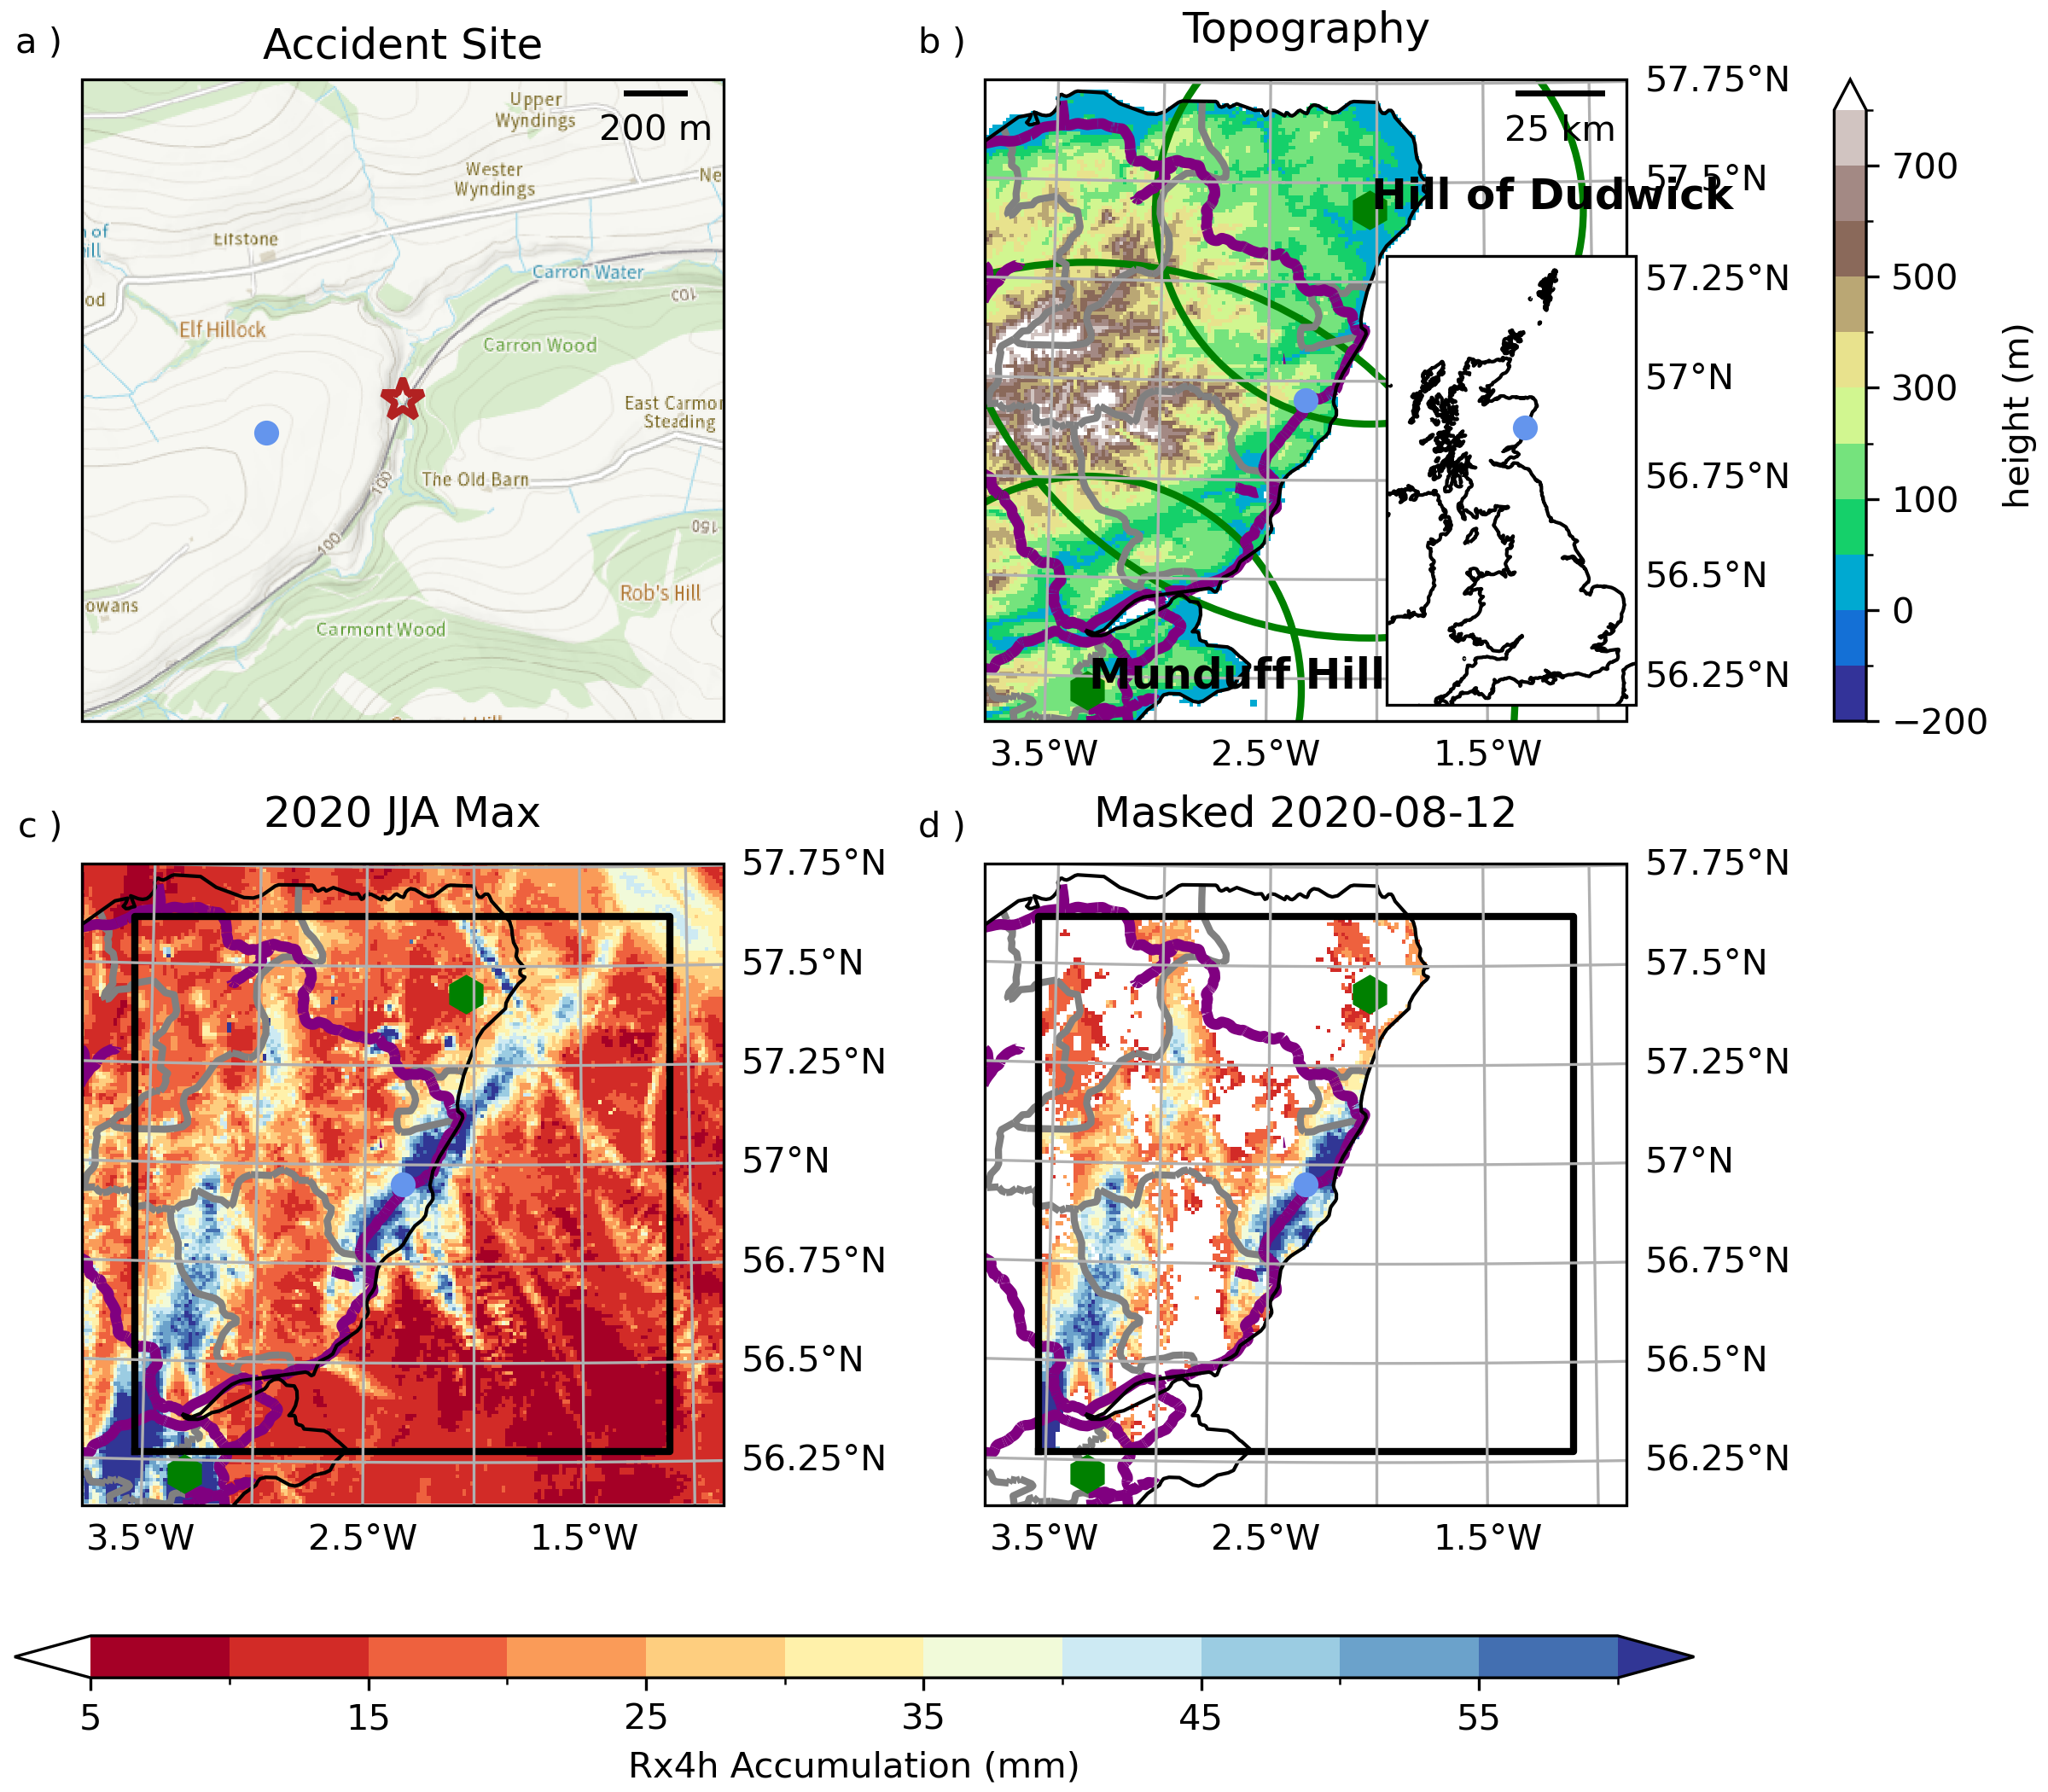
\includegraphics[width=\linewidth]{carmont_geog_group.png}
	\caption{a) Topography of North East Scotland (at 1km resolution). Also show, by their first two letters, are locations of Dyce, Aviemore, Aberdeen, Stonehaven and Montrose. Inset shows Great Britain and Ireland. Colour scale on bar to right. Circles are  60 and 120 km from radar stations (green hexagons with full names). b)  Map of Carmont Accident site -- brick red star shows where train derailed. Main features are contour lines every 10 meters, railway (black line) and woods (green) (Map crown copyright Ordinance Survey).  c) Maximum 4 hour radar rainfall accumulation  for JJA 2020. d) Event of 2020-8-21.  Black box in c \& d shows 150x150 km region of interest. Scale bars are shown in a and b. Location of Carmont drain shown in all plots as pale blue dot.  }
	\label{fig:carmont_geog_group}
\end{figure}

\begin{figure}[tp]
	\centering
	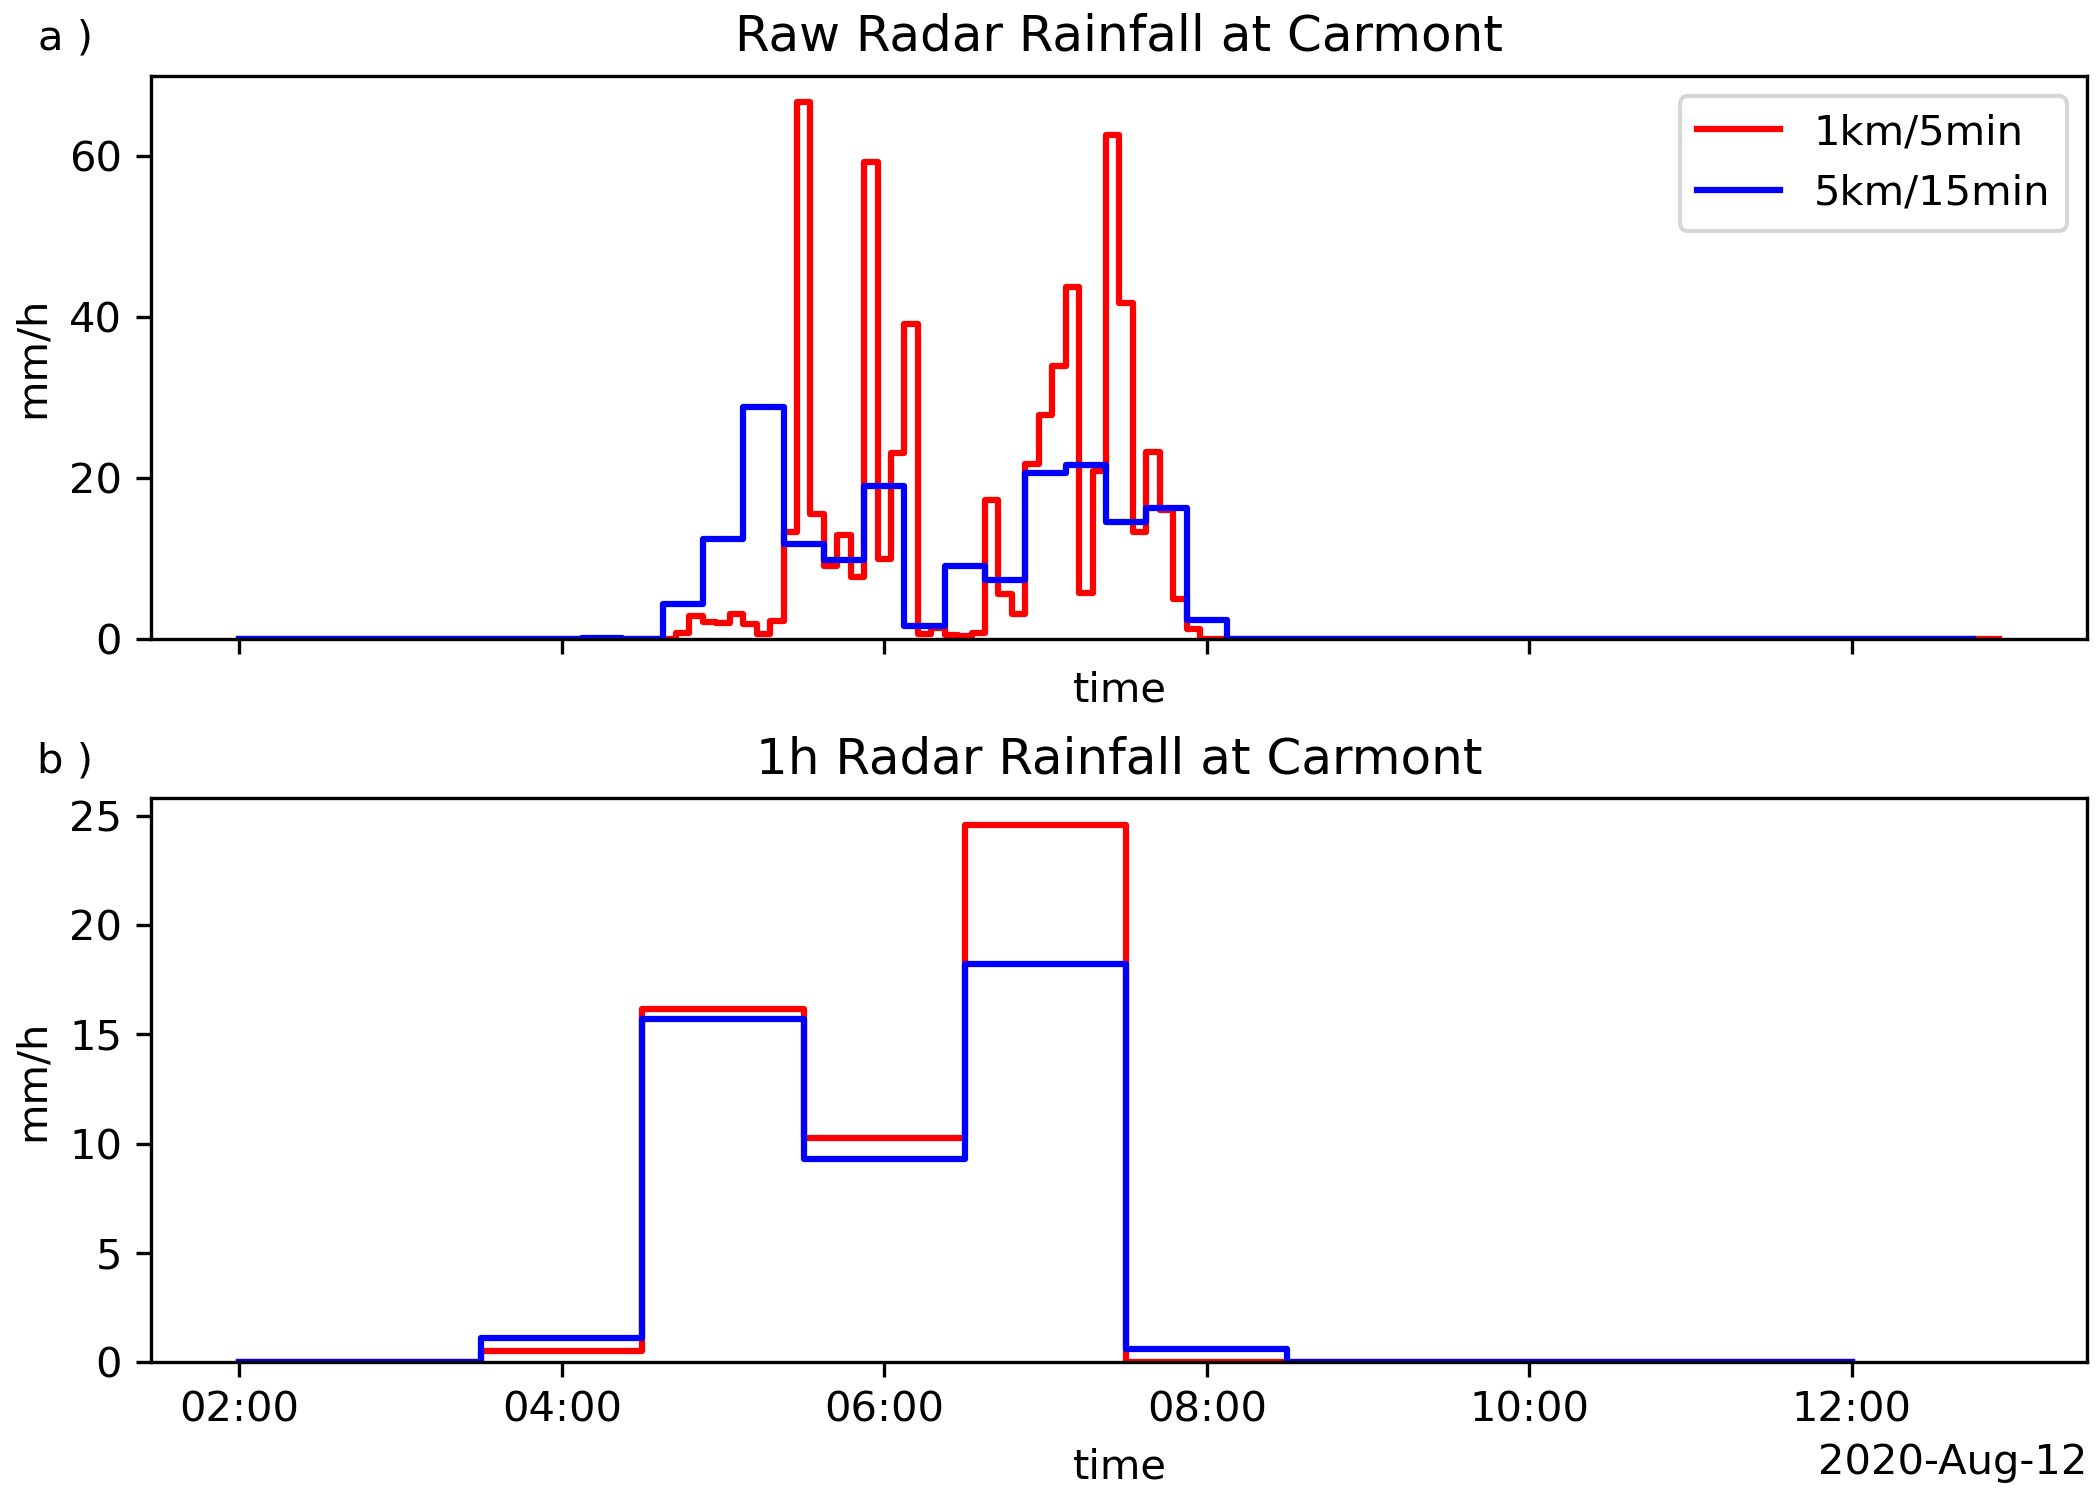
\includegraphics[width=0.5\linewidth]{radar_carmont.png}
	\caption{a) Radar rainfall rates at Carmont (mm/h) for 1km/5 min (red) and 5km/15 min. Dotted lines show accumulation reaching 51.5 and 44.9 mm for the 1km \& 5km data respectively. Circles show when 1/2 the total rain has fallen; b) Hourly mean rates for 1km (red) and 5km (blue) radar data. Data is shown from 2020-08-12T02:45 to 10:15 and ``Derail'' shows when the train derailed. }
	\label{fig:aug2020_rain}
\end{figure}




\begin{figure}
	\centering
	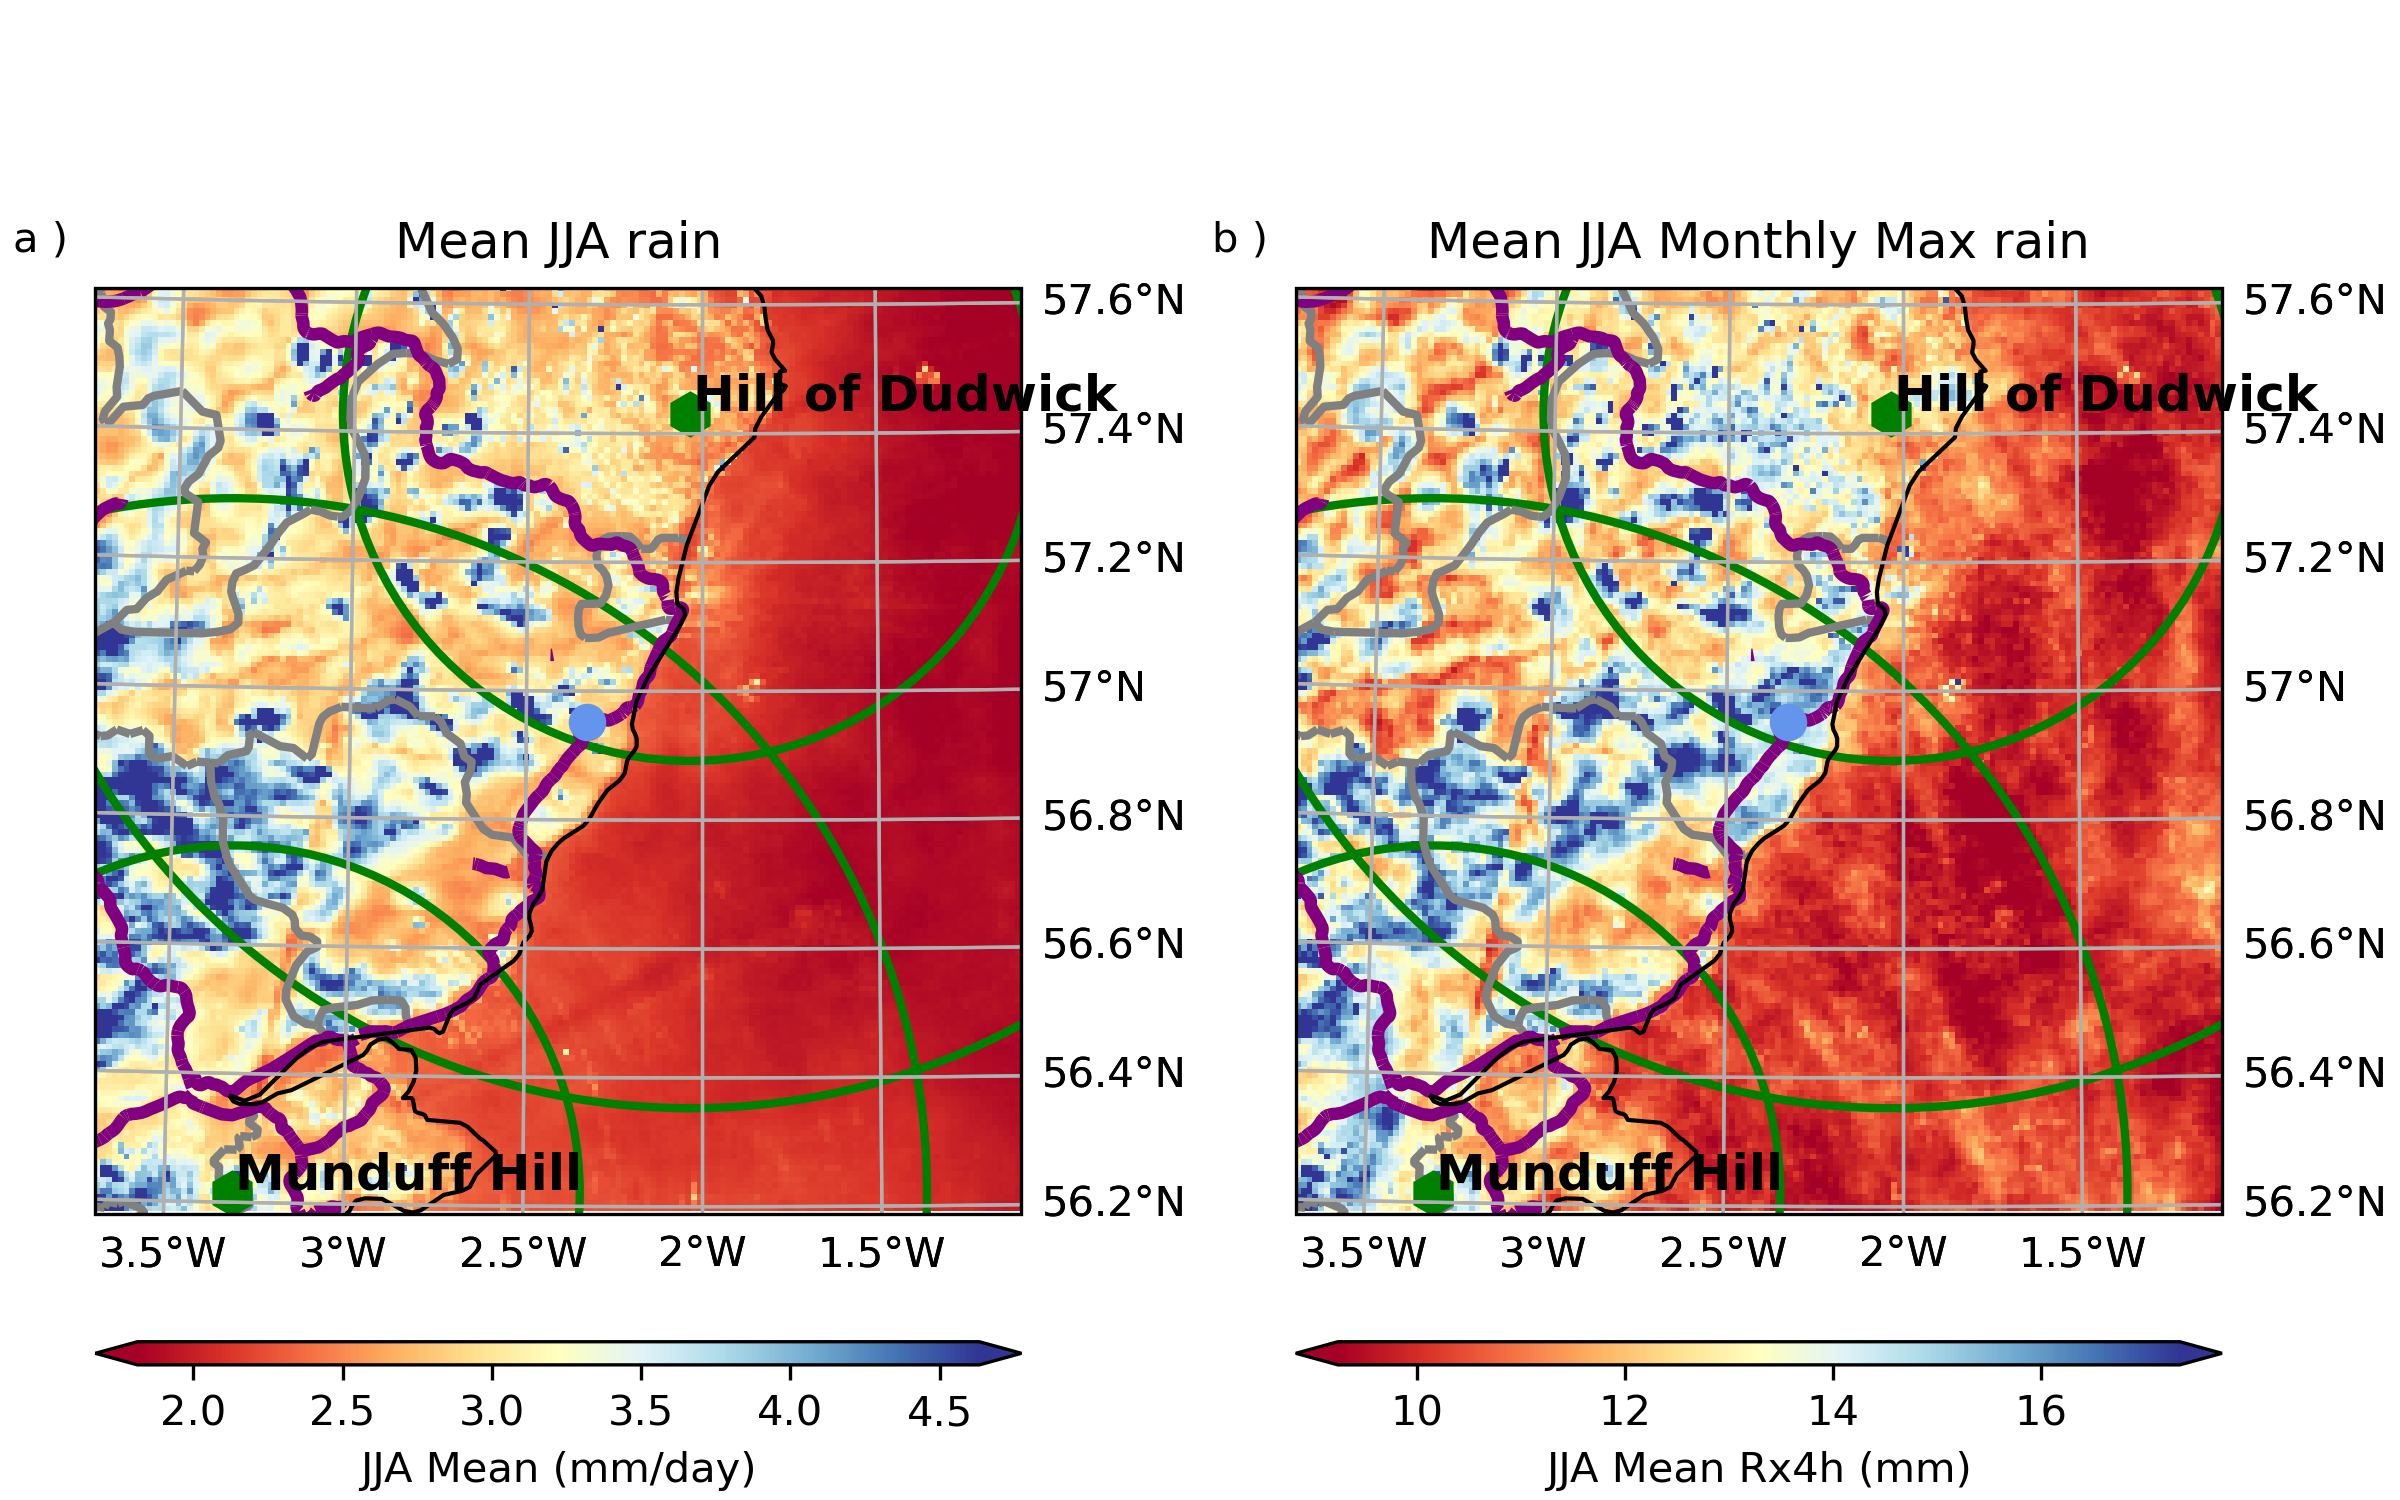
\includegraphics[width=\linewidth]{radar_jja}
	\caption{a) Mean radar rainfall (mm/day) b) Mean monthly maximum 4h rain total (mm/h). Means are for summers (June-July-August) from 2008 to 2023 inclusive. Circles are  60 and 120 km from radar stations (Green hexagons). Pale blue circle shows point ("Carmont drain") where rain occurred, purple lines show railways and grey lines local authority boundaries. }
	\label{fig:mean_rain}
\end{figure}


\begin{figure}[tp]
	\centering
	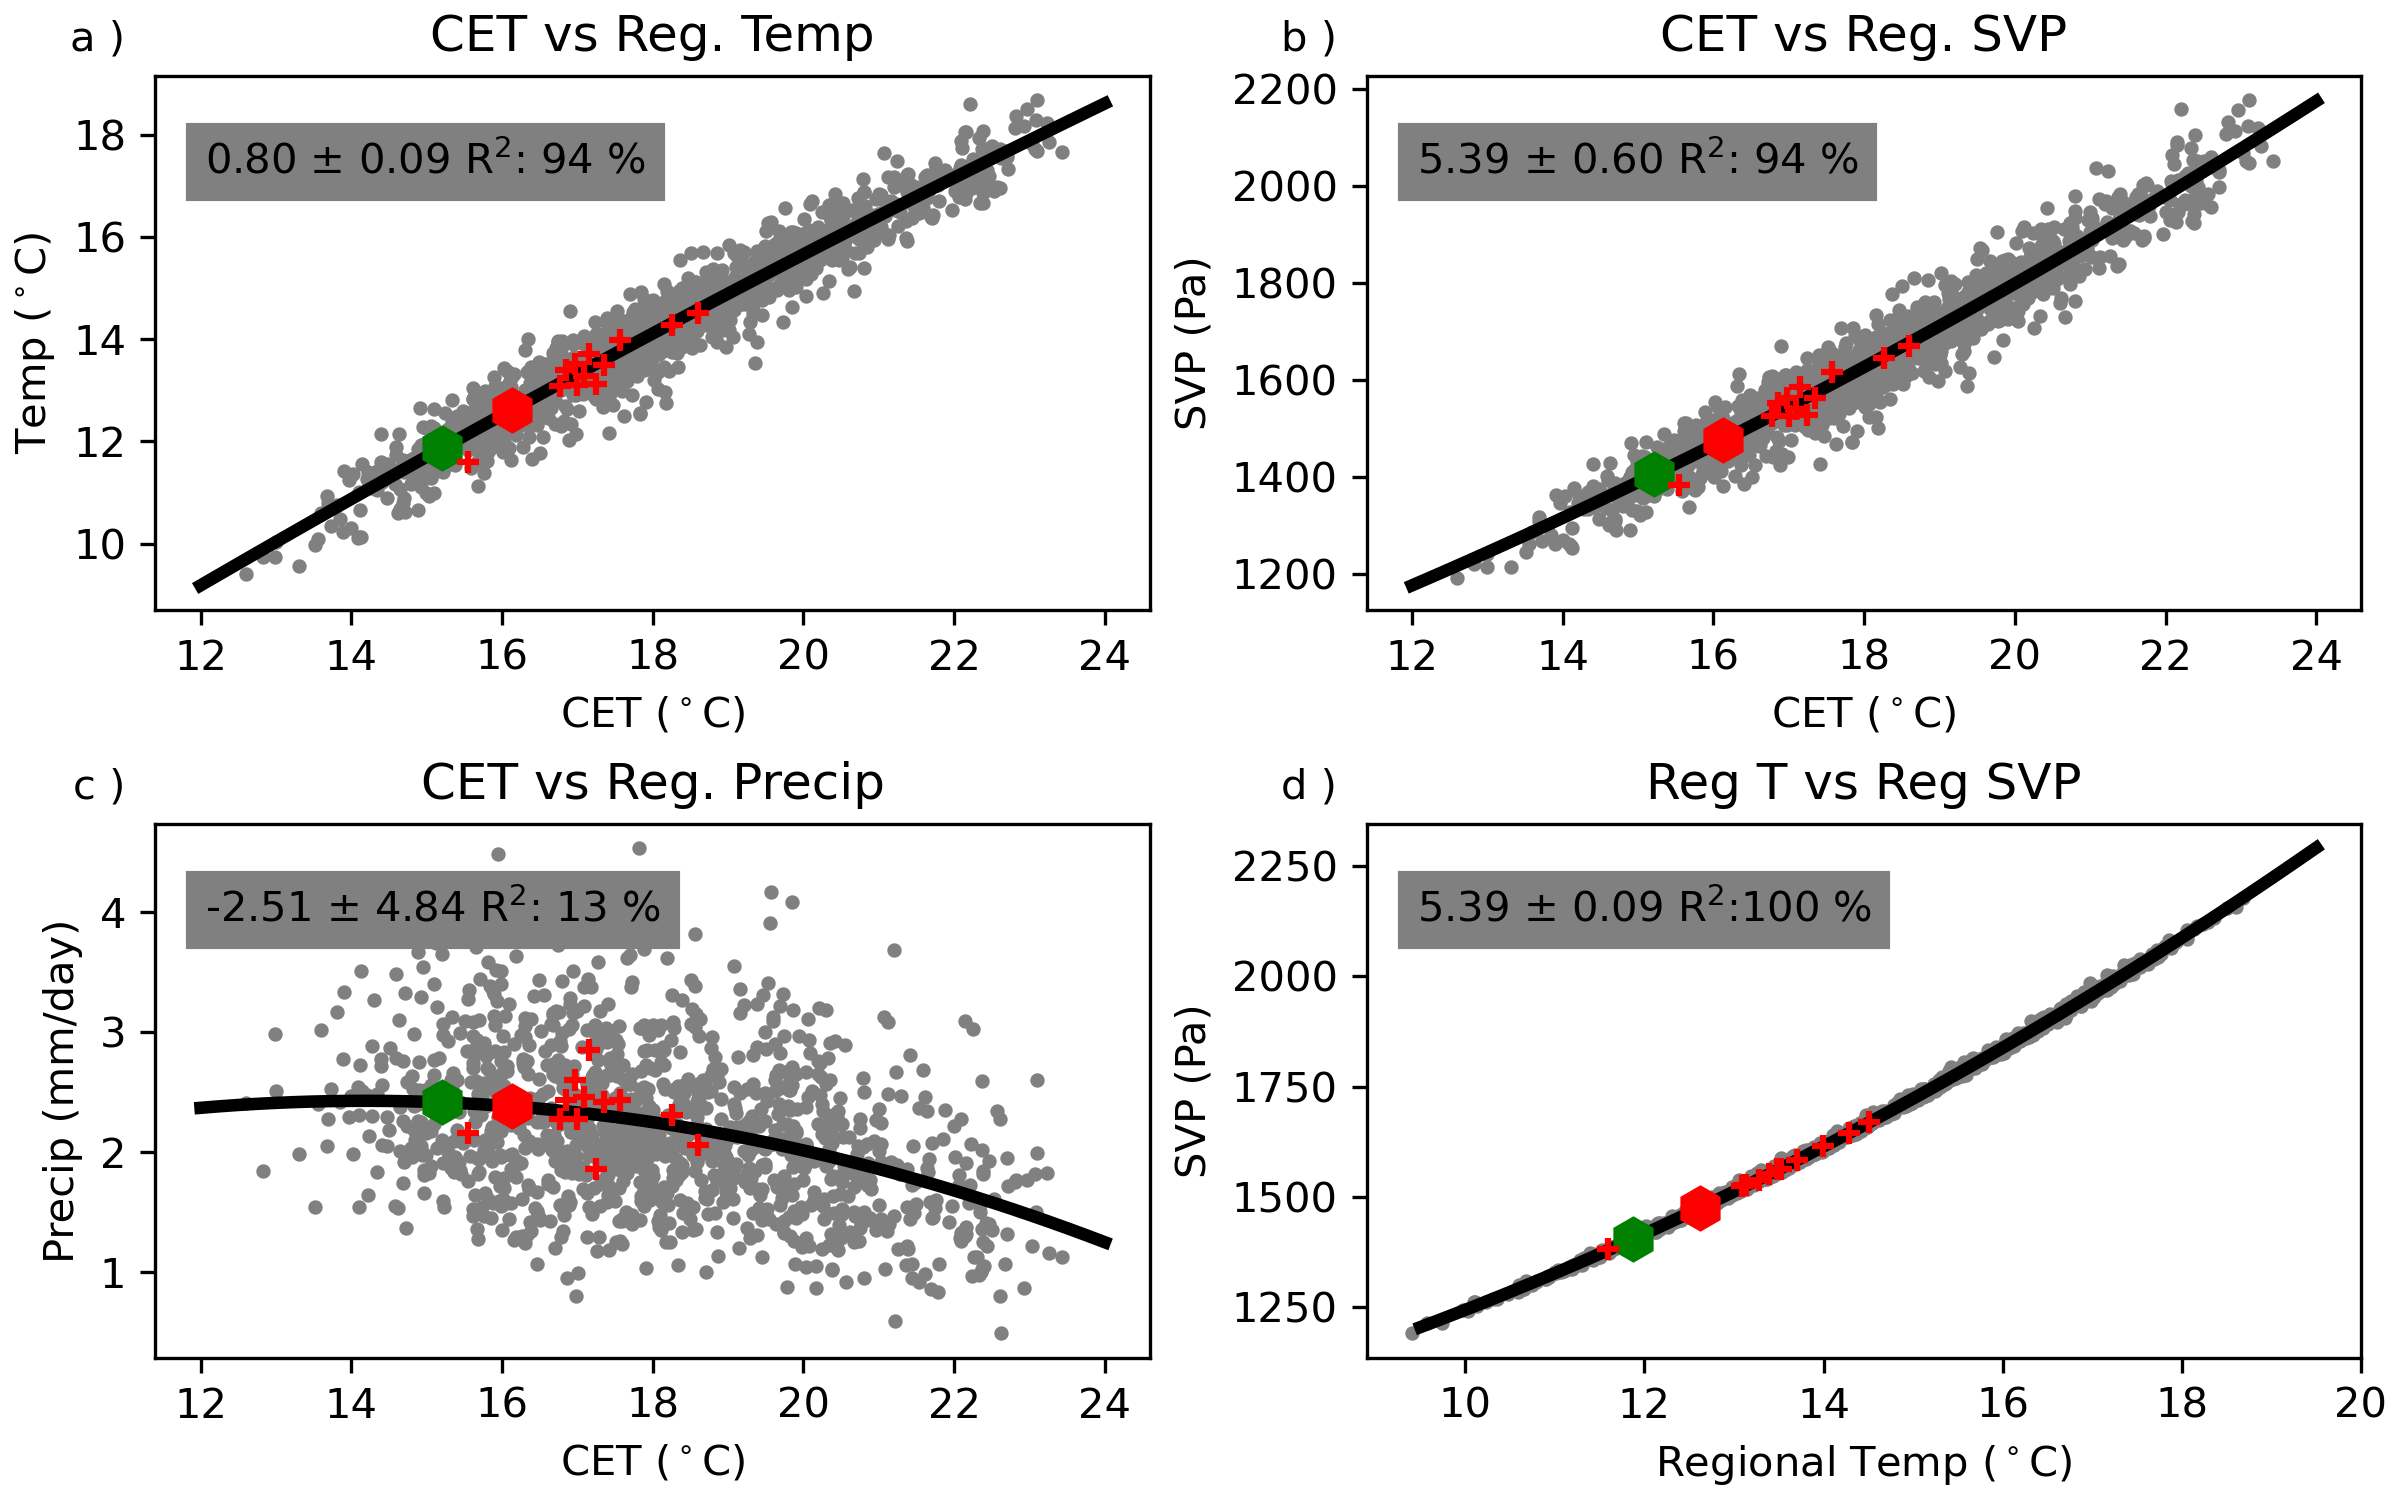
\includegraphics[width=\linewidth]{scatter.png}
	\caption{Scatter plots for summer mean  a)  Central England Temperature (CET) vs  regional mean temperature; b) CET vs regional average saturated vapour pressure (SVP); c) CET vs regional average precipitation; d) Regional temperature vs Regional SVP. Green and red hexagons show estimated 1850-1899 and 2012-2021 average values. Lines show second order best fits.}
	\label{fig:cet_scatter}
\end{figure}

\begin{figure}
	\centering
	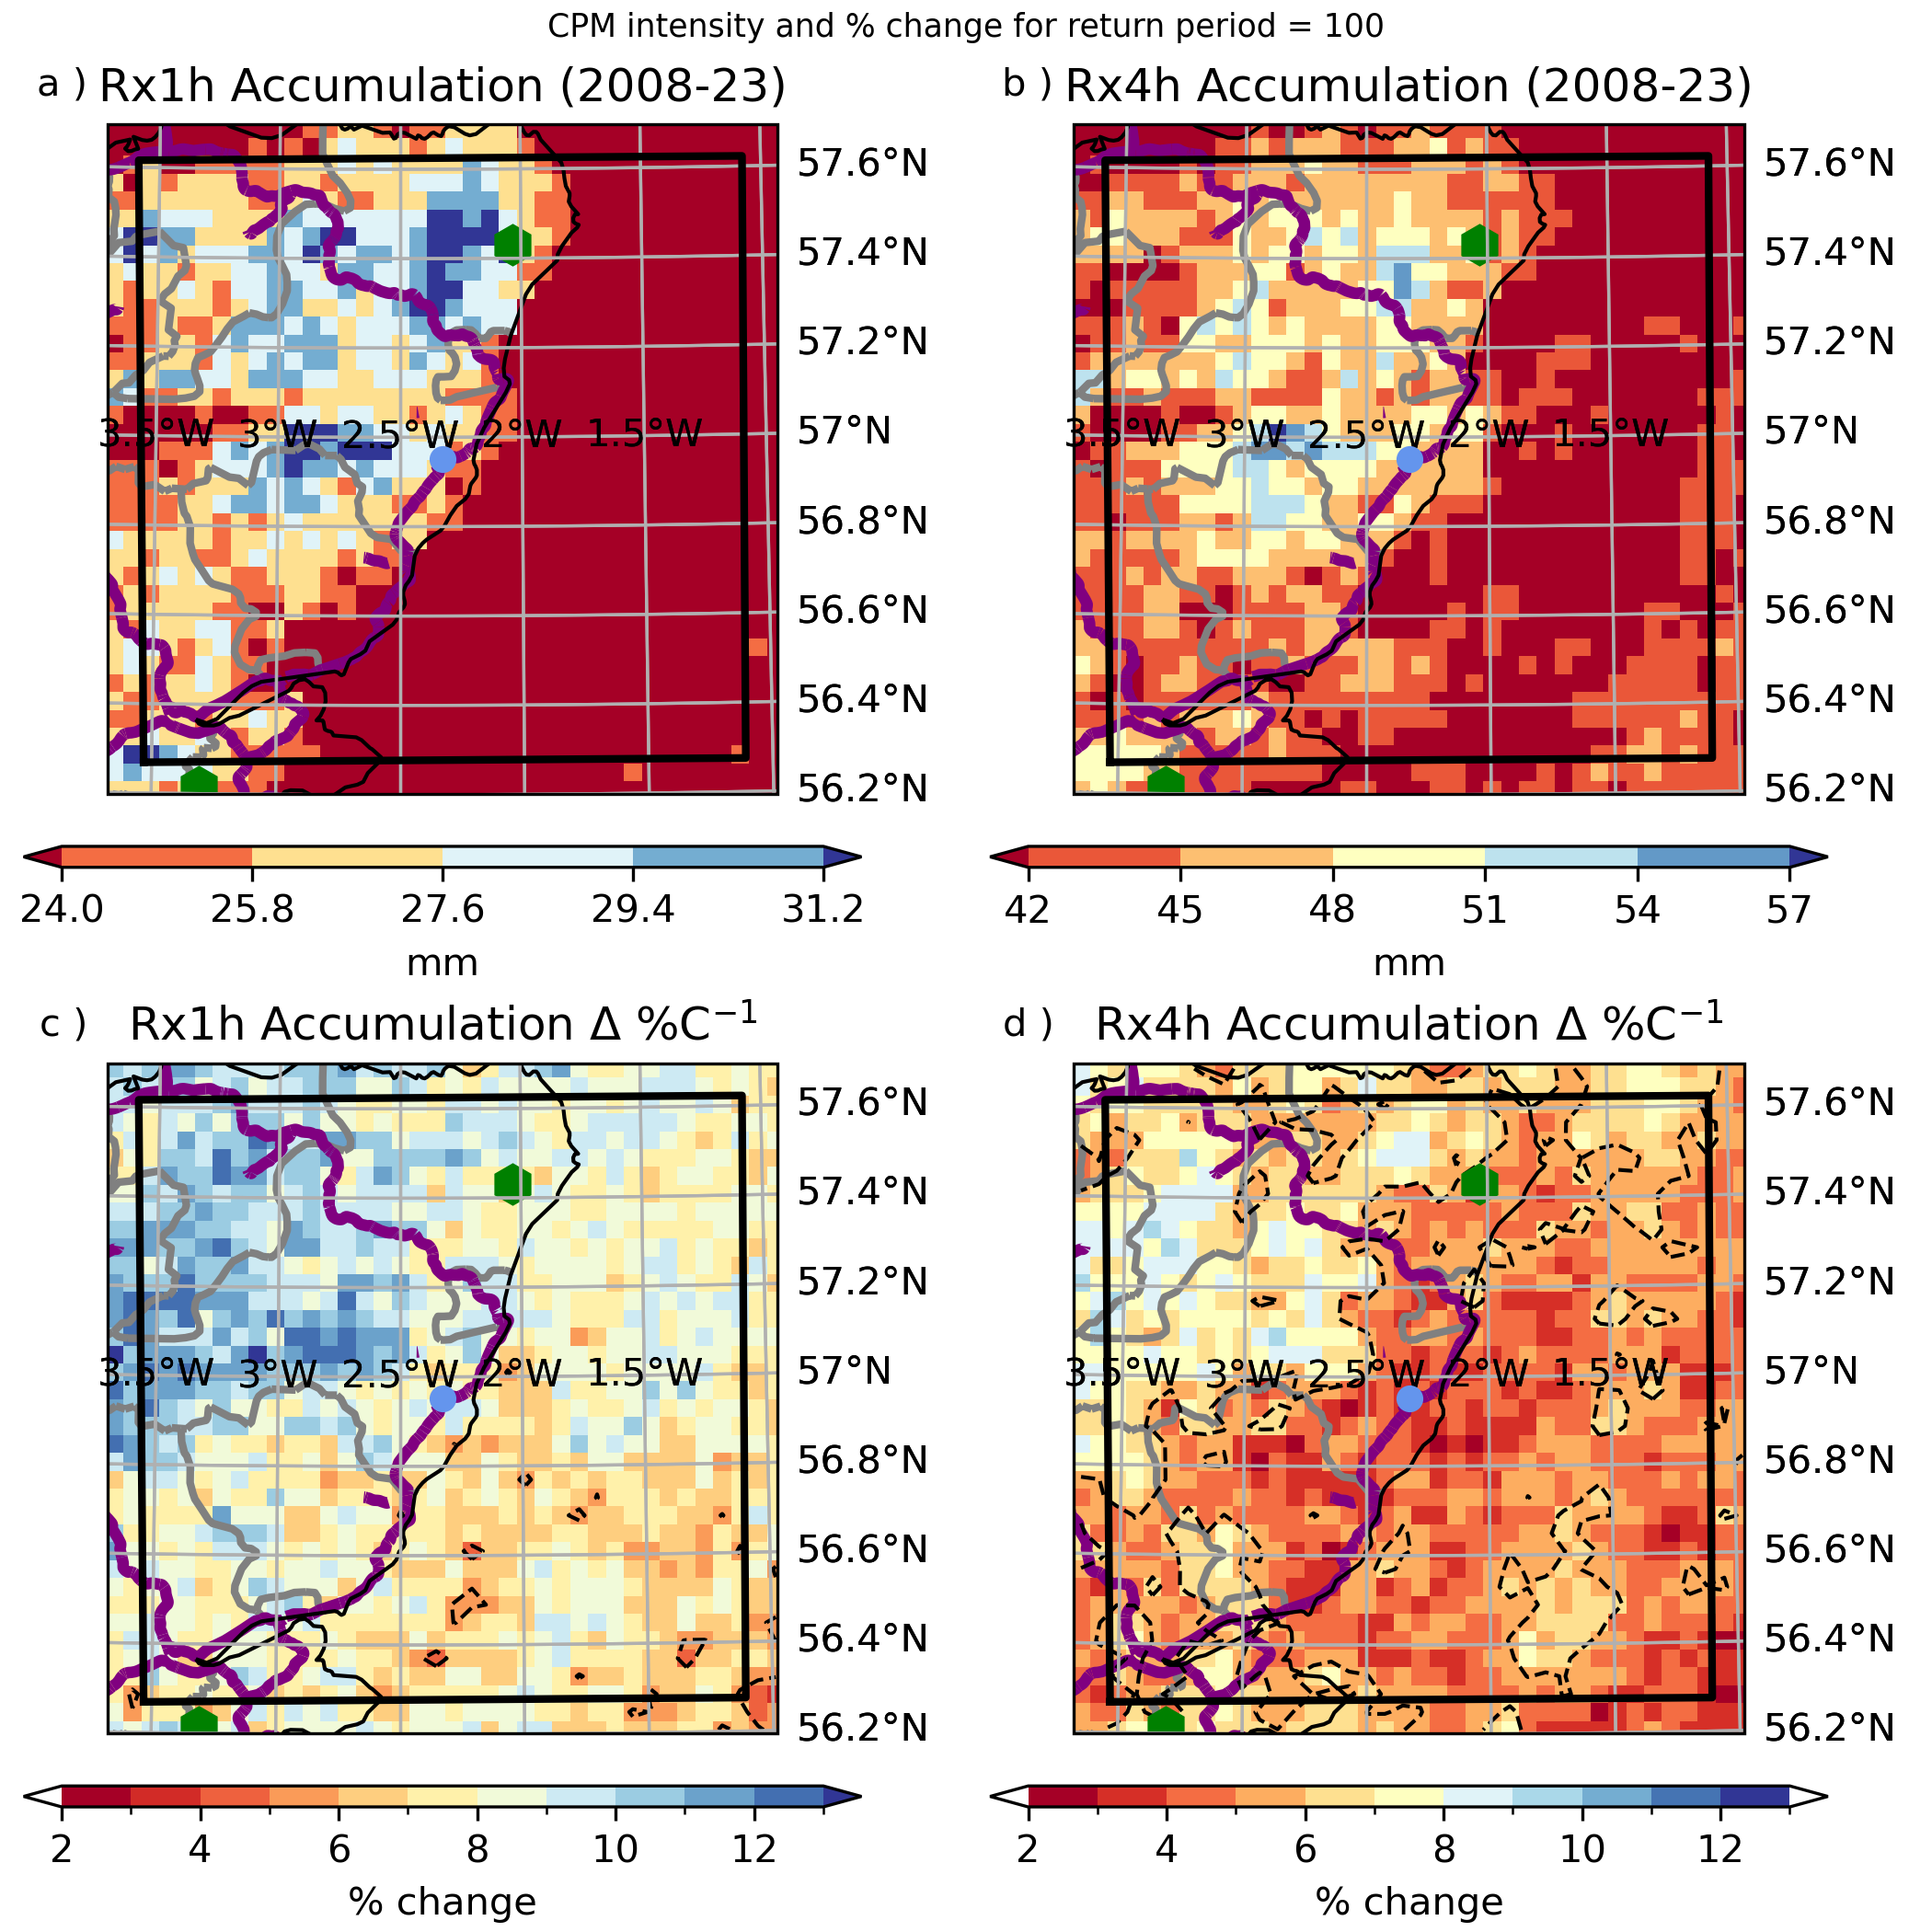
\includegraphics[width=1\linewidth]{cpm_intensity_delta}
	\caption{One in a hundred year CPM maximum rainfall accumulation for 1 and 4 hour rainfall (a \& c) and percentage sensitivity to 1 degree CET increase. Dashed lines shows intensity increase of 5.4\%/degree CET corresponding to CC. Other elements as Figure~\ref{fig:mean_rain}.  }
	\label{fig:map_intensity}
\end{figure}

\begin{figure}
	\centering
	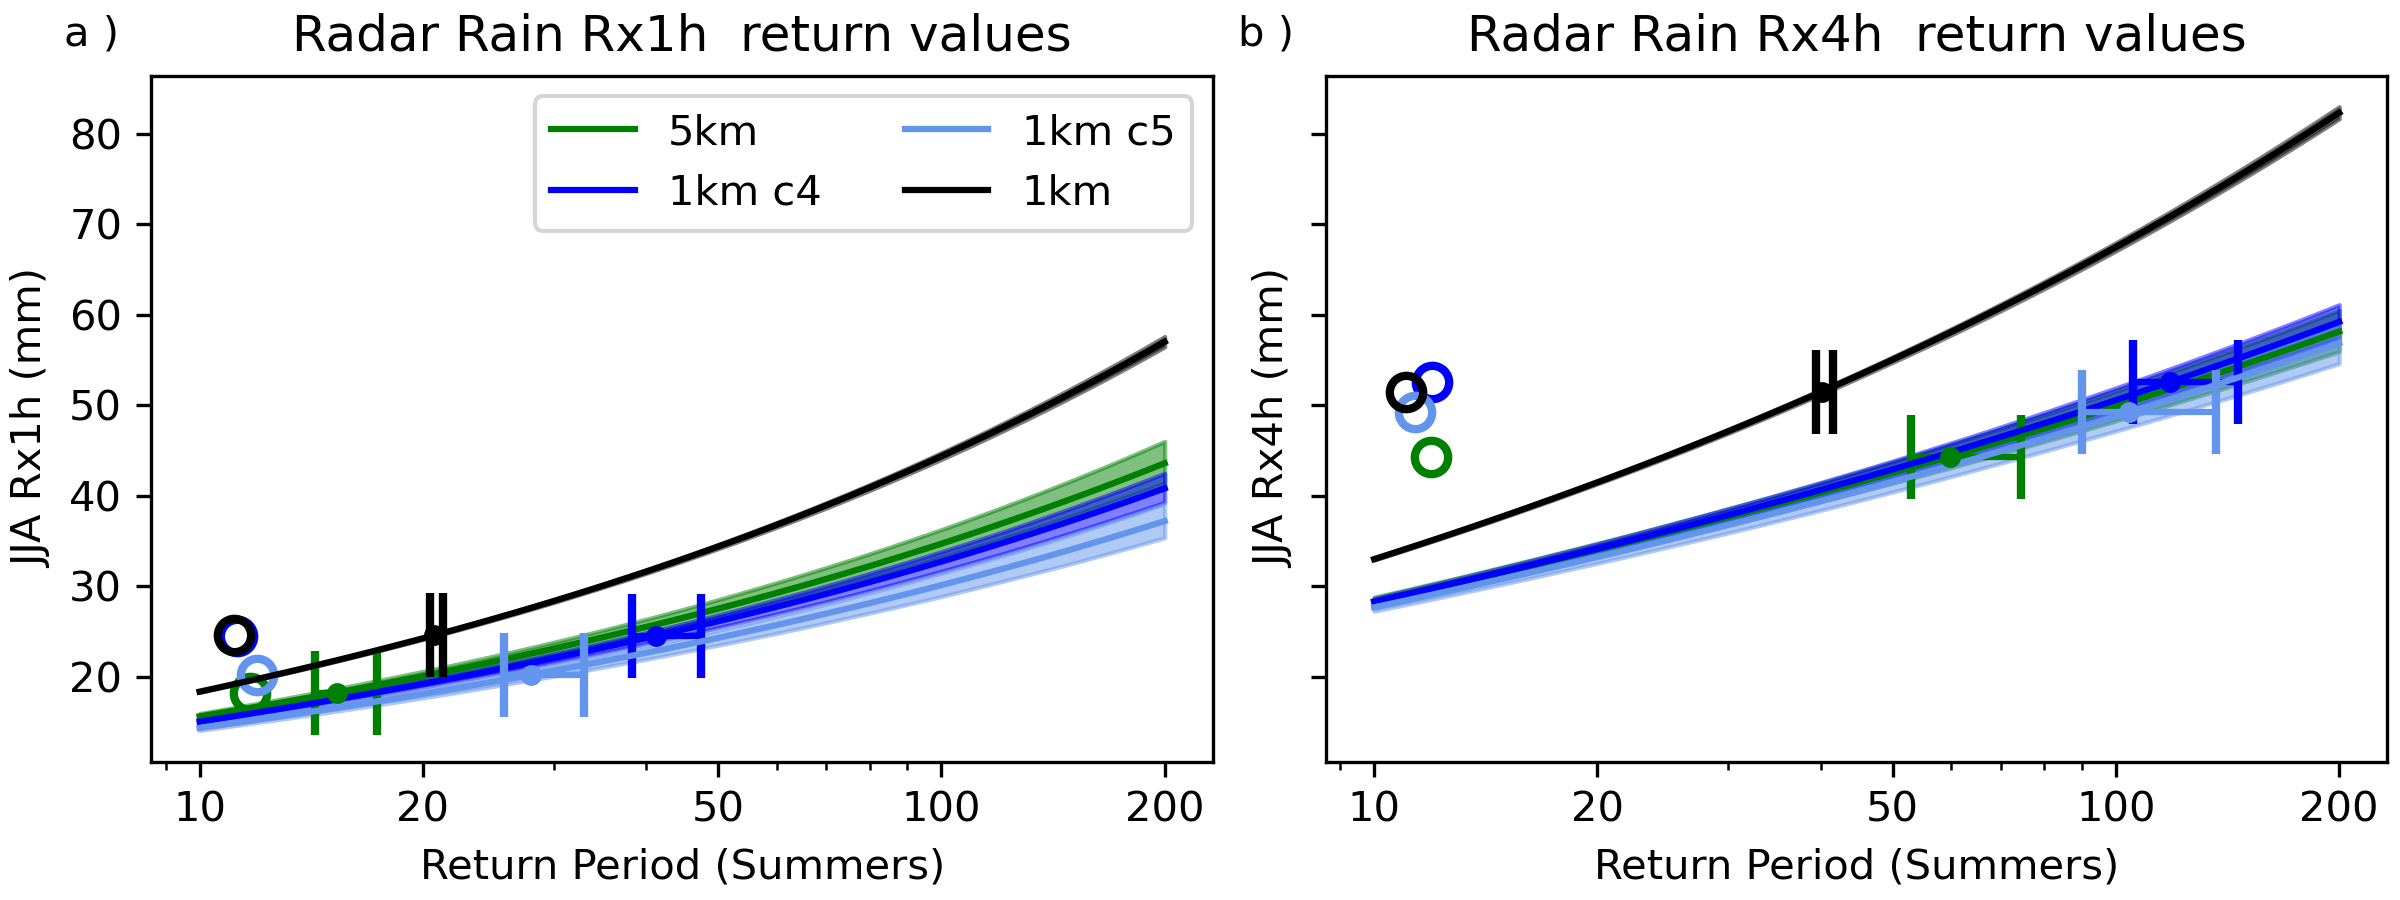
\includegraphics[width=\linewidth]{radar_return_prds}
	\caption{Estimated return values for  JJA maximum accumulated radar rainfall. Shown are Rx1h (a) and Rx4h (b) for 1km  (black),  5km (green), 1km-c4 (blue) and 1km-c5 (pale blue) radar rain. Symbols in left hand of sub plots show radar rain at nearest gridpoint to Carmont drain. Horizontal error bars show return periods range for those values. }
	\label{fig:radar_rtn_prd}
\end{figure}

\begin{figure}
	\centering
	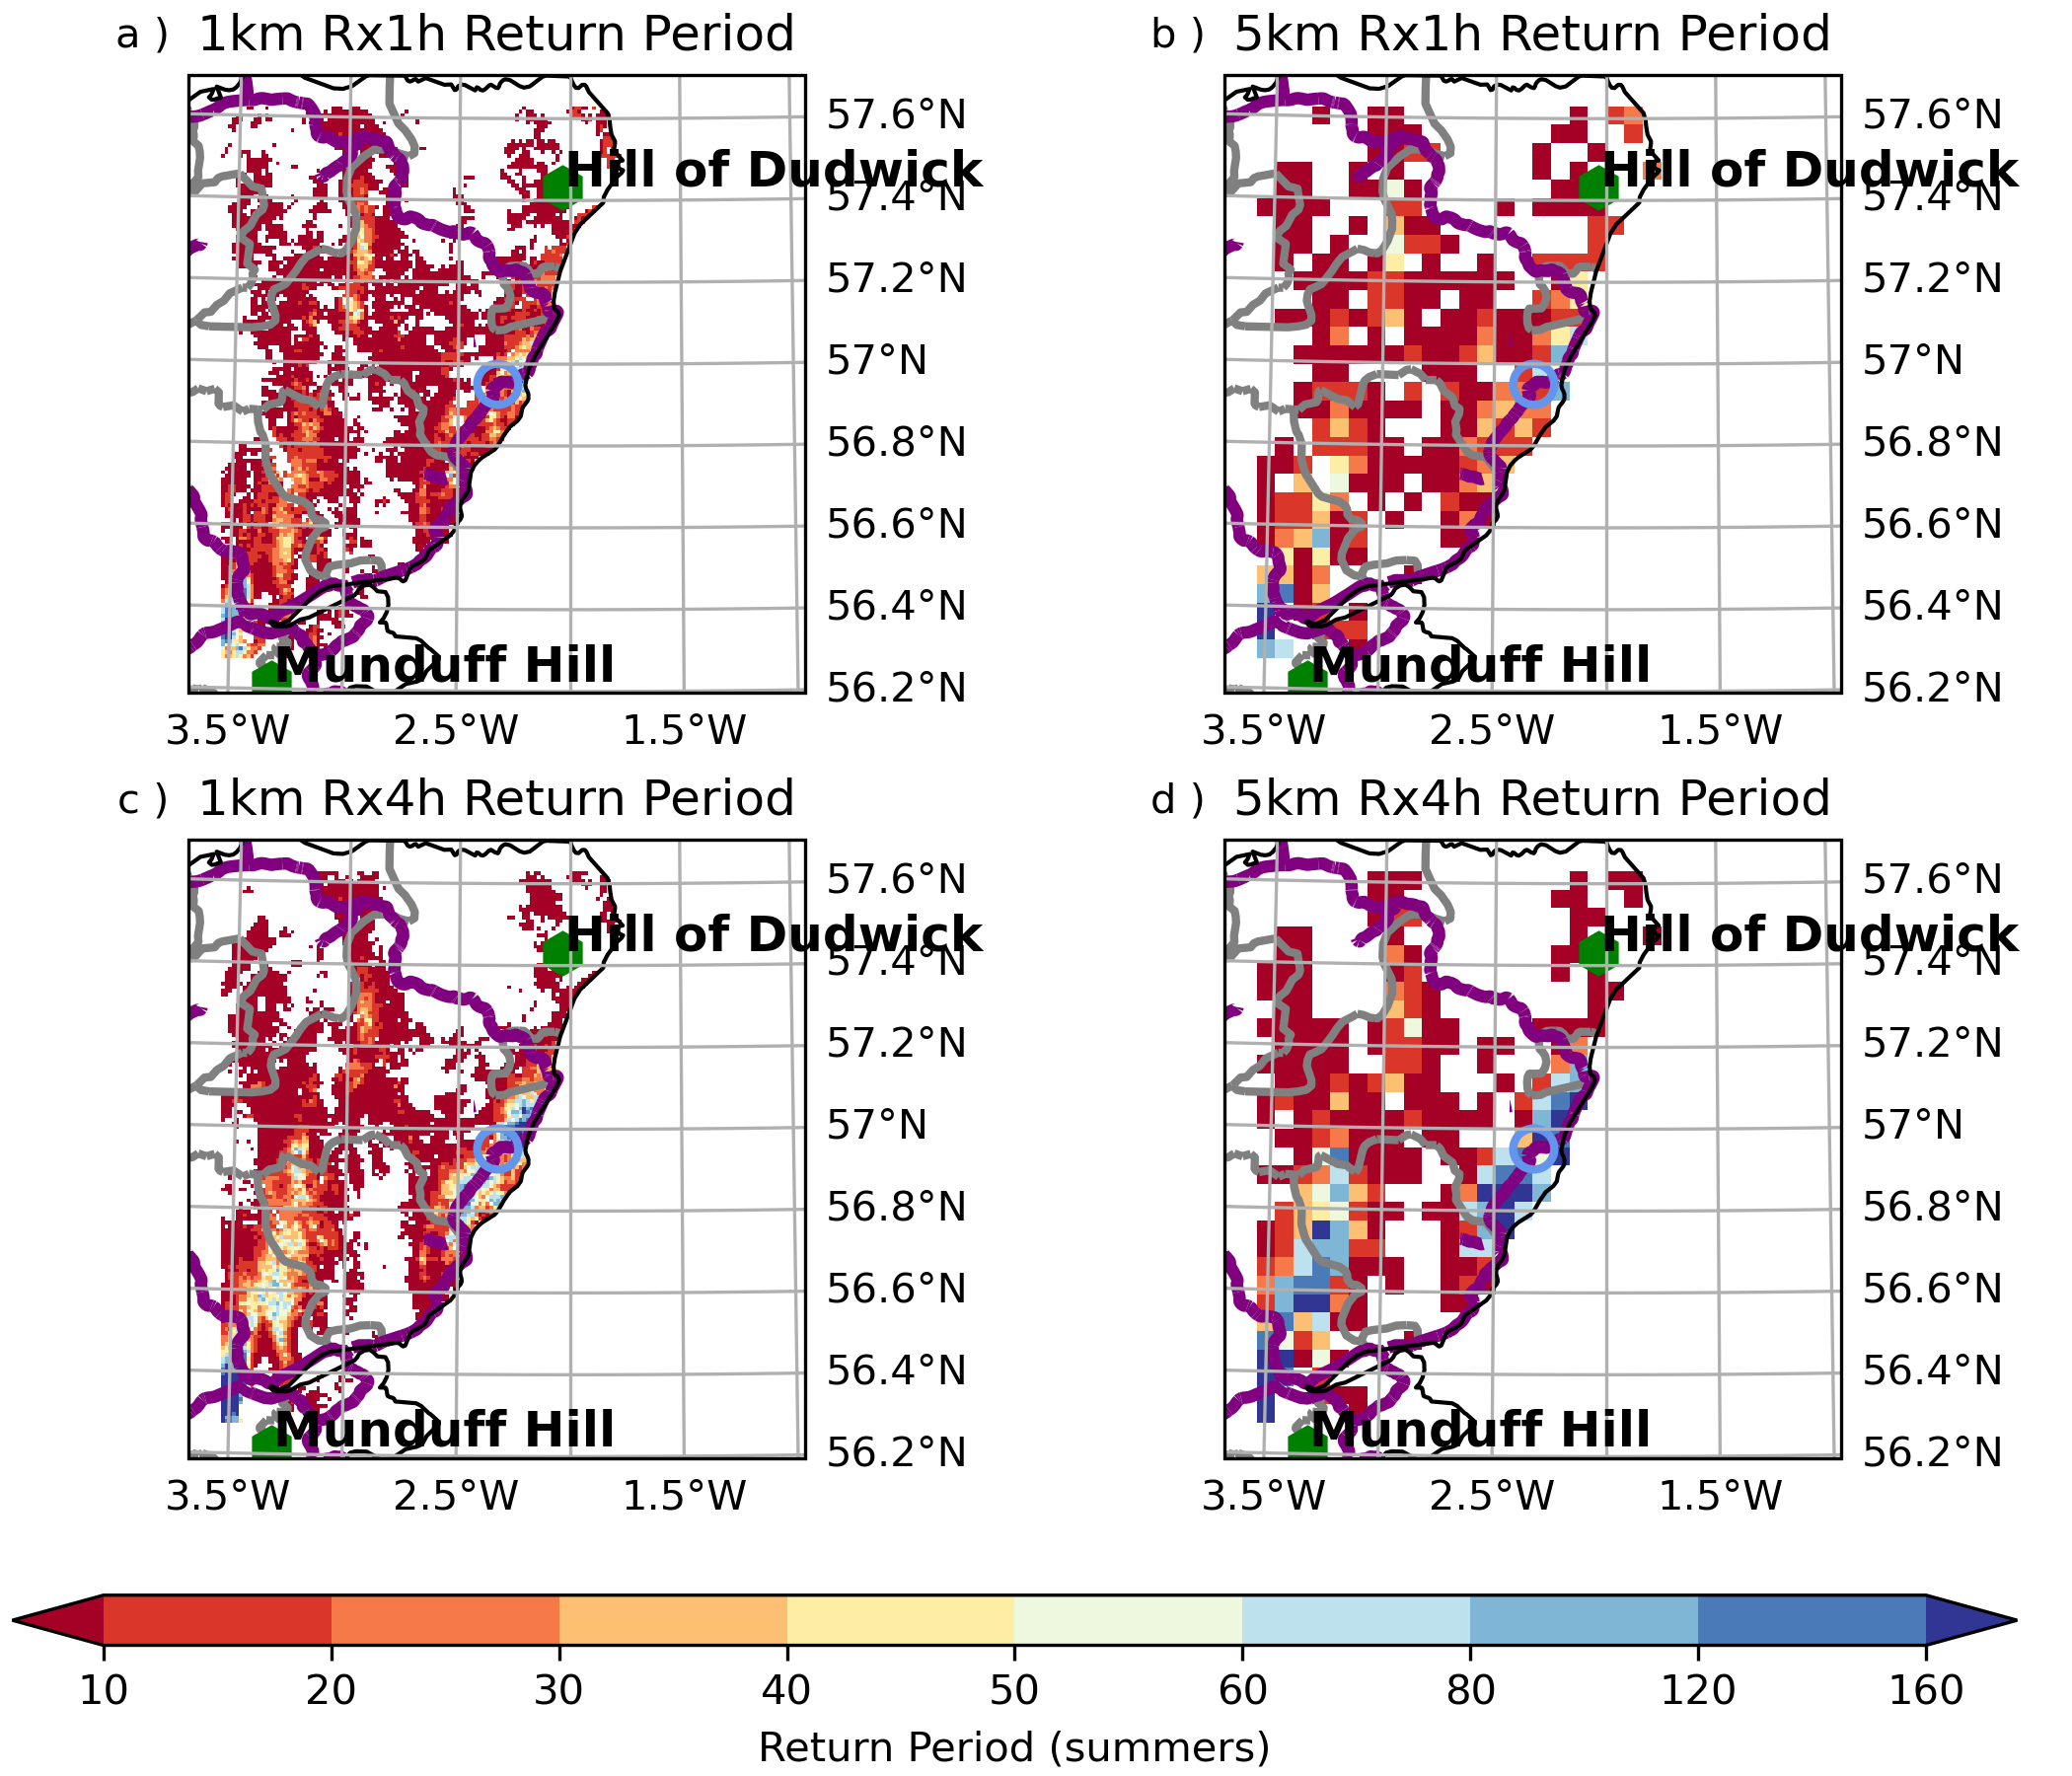
\includegraphics[width=\linewidth]{map_return_prds}
	\caption{Best estimate Return periods for Carmont region. Plots a \& b show Rx1h while plots c \& d show Rx1h. Color bar at bottom refers to all plots. Other elements as Figure~\ref{fig:mean_rain}. } 
	\label{fig:map_rtn_prd}
\end{figure}


\begin{figure}
	\centering
	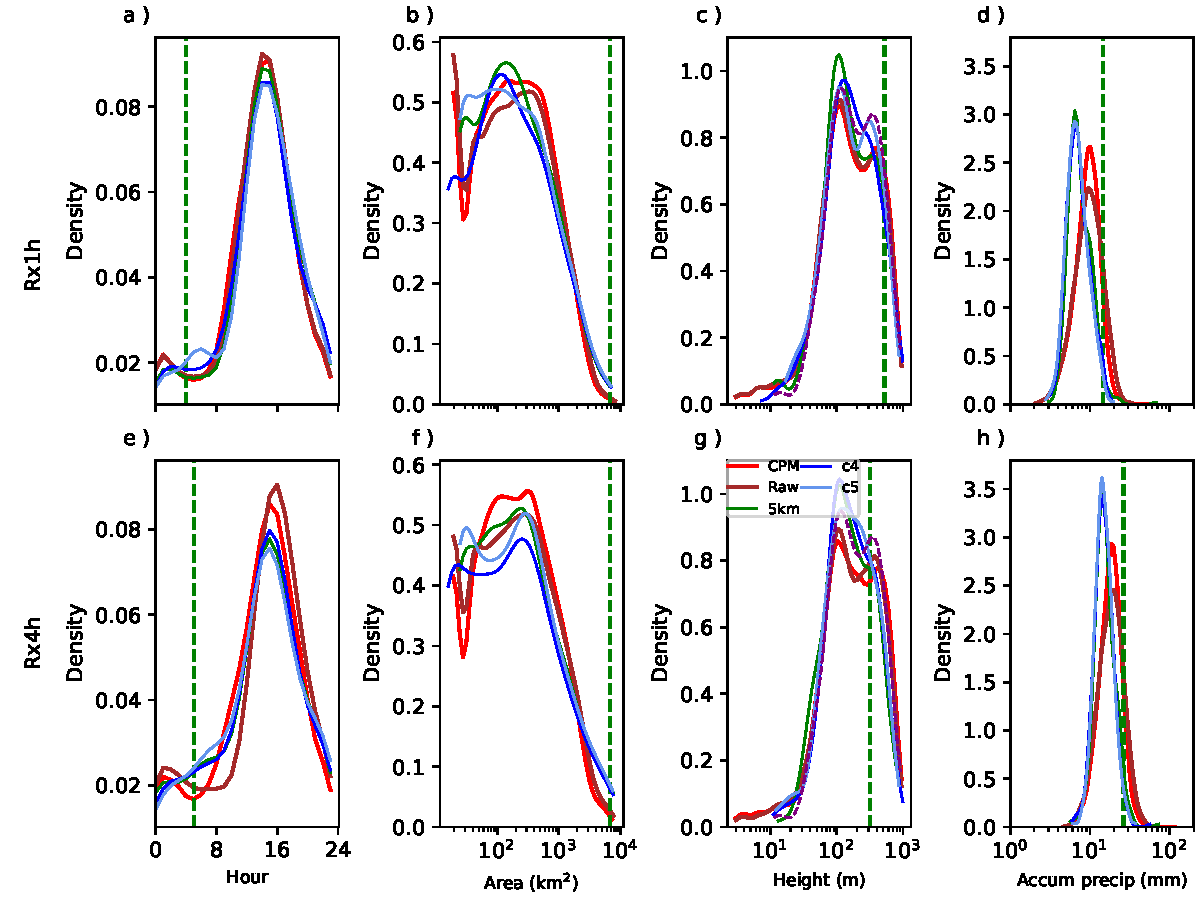
\includegraphics[width=\linewidth]{kde_smooth_events}
	\caption{Kernel Density Estimates from  CPM (orange), CPM-Raw (brown), 5km radar (green), 1km-c4 (blue) and 1km-c5 (pale blue) events at 50\% quantile for 2008-2022 period. Shown are day-hour (a \& e),$\log_{10}$ of event area (b \& f),  topographic height (c \& g ) and maximum Rainfall accumulation (d \& h). Top row shows Rx1h while bottom row shows Rx4h values.}
\end{figure}




    
%    \begin{figure}
%    	\centering
%    	\includegraphics[width=\linewidth]{fit_ratio.png}
%    	\caption{a) \% change per degree CET change in location parameter between 2061-2080  and 1981-2000 for all events in the filtered UKCP ensemble. b) as a) but for scale parameter. c) Shape parameter for 1981-2000 (blue) and 2061-2018 (orange) data. All results are shown as a function of event quantile and errors bars are $\pm2\sigma$. Dotted lines in a) \& b) show mean value of the parameter. Dashed horizontal line in c shows shape value of 0.}
%    \end{figure}


\begin{figure}
	\centering
	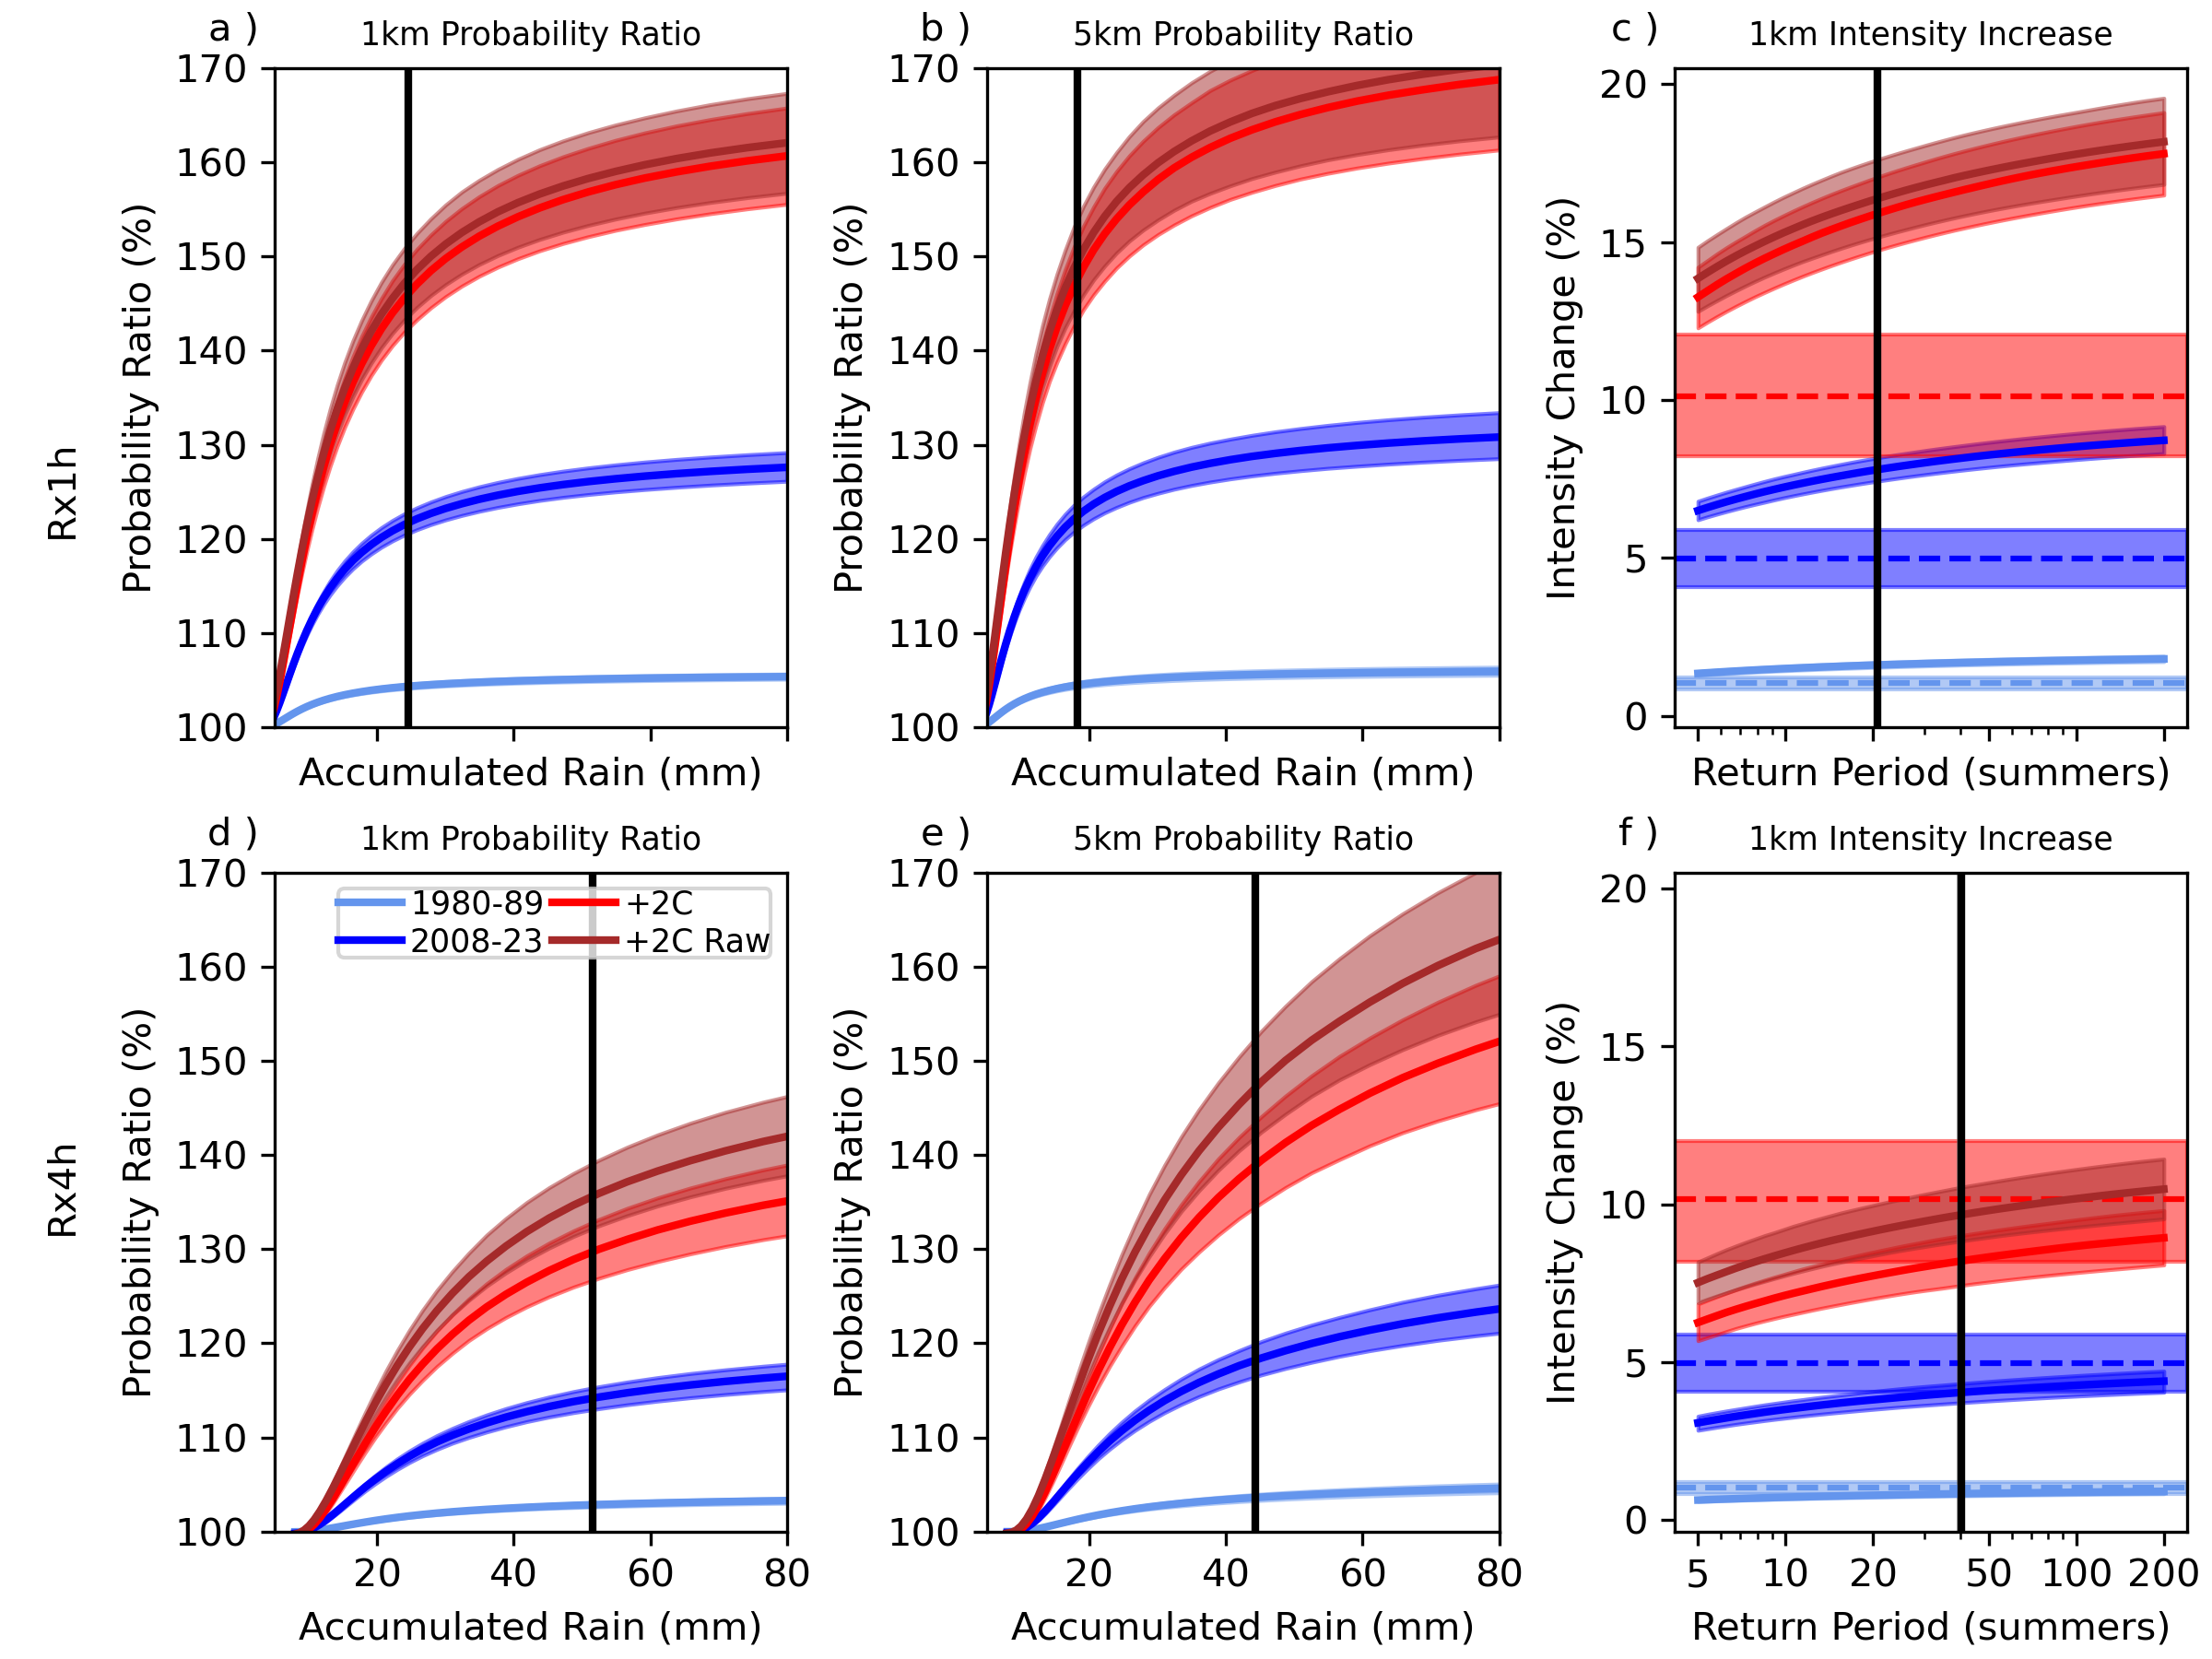
\includegraphics[width=1\linewidth]{intens_prob_ratios}
	\caption{a \& d: Probability ratio, relative to Pre-industrial, at Carmont drain as function of accumulated rainfall for 1km radar rainfall. b \& e) As a but for 5km radar rainfall. c \& f: Intensity ratio at Carmont drain  as function of  return period. Also shown are median (horizontal dashed line) and 5-95\% uncertainties (vertical shading) for changes expected from Clausius-Clapyron. Upper plots (a-c) show Rx1h accumulations while lower plots (d-f) show Rx4h accumulations. All plots show changes for +2C world (red), 2012-2021 (dark blue) and 1980-1989 (pale blue) from filtered CPM data. Brown shows changes in +2C world when raw CPM data is used.   Solid lines are median changes with 5-95\% uncertainty range shown by  shading.}
	\label{fig:int_pr}
\end{figure}

\begin{figure}
	\centering
	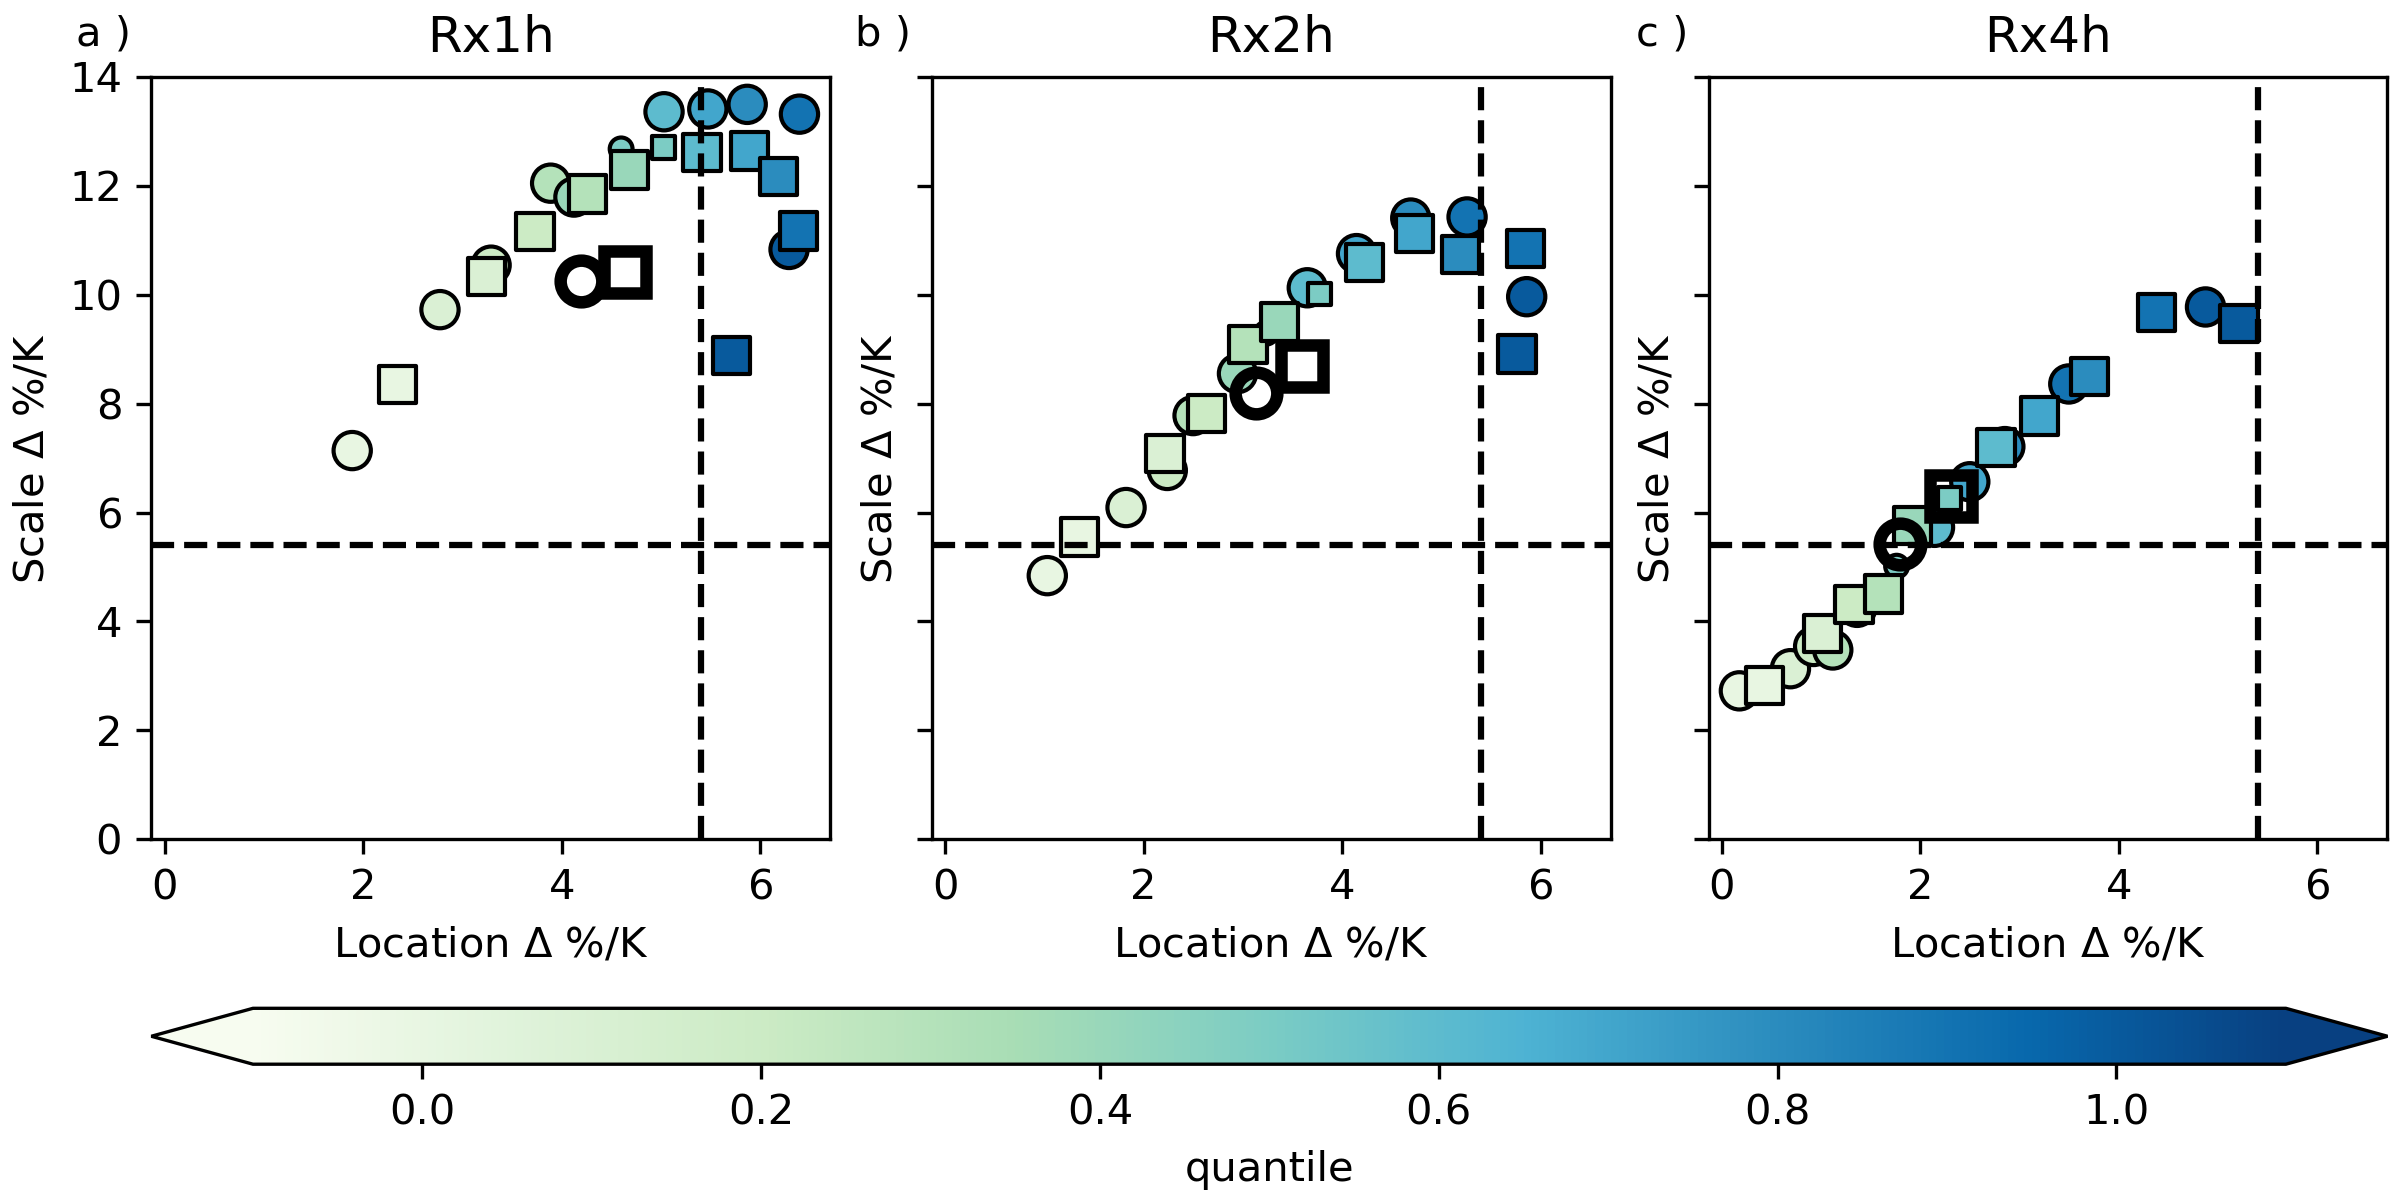
\includegraphics[width=\linewidth]{carmont_gev_quant_change}
	\caption{Fractional change in GEV scale  and location parameters for raw (squares) and filtered (circles) CPM data. Colours denote quantiles in 5x5 region (approximately 22x22 km) centred on Carmont Drain. Small symbols show where change is not significantly different from median quantile change. Dashed horizontal and vertical lines show mean Clausius-Clapeyron changes. Black symbols show fractional change for the whole region.  Show are Rx1h (a), Rx2h (b) and Rx4h values.}
	\label{fig:carmon_gev_quant_change}
\end{figure}

\end{document}
